\section{Choice of SB/CR defintions} %updated May 15 2017
\label{app:SB-optimization}

\paragraph{}
This section is for detailed description of Sideband and Control region choice, for Section~\ref{sec:boosted-SBCR}.

\paragraph{} 
Sideband size is limited to be outside the control region. The choice of the upper bound of the Sideband is constrained such that the leading jet mass spectrum will contain the \ttbar peak and so that the Sideband has enough statistics and is as close to the signal and control region as possible. One test is to vary the Sideband size and to re-estimate the $\mu_{\text{qcd}}$ and $\alpha_{t\bar{t}}$ values. This is shown in Figure ~\ref{fig:app-sb-muqcd-diffSB}. The values of fitted $\mu_{\text{qcd}}$ and $\alpha_{t\bar{t}}$ are fairly stable for different Sideband choices.

\paragraph{} 
To evaluate the statistical effect of smaller Sideband regions, we plot the ratio of the stat uncertainty of the predicted number of events vs. the fit uncertainty of $\mu_{\text{qcd}}$ and $\alpha_{t\bar{t}}$. This is shown in Figure ~\ref{fig:app-sb-muqcd-diffSB}. In Sideband region, the ratio (right) is close to 1, because the Sideband normalization is fixed in the fit. Based on the choice that for the signal region predictions, the fit uncertainty should be around half of the statistical uncertainty, the Sideband upper limit is chosen to be $R_{hh}^{\text{high}} < 58$ \GeV. Note that this will be the way to assign non-clusure test in the systematics, as described in Section~\ref{sec:non-closure-mu-qcd}.

\begin{figure*}[htbp!]
\begin{center}
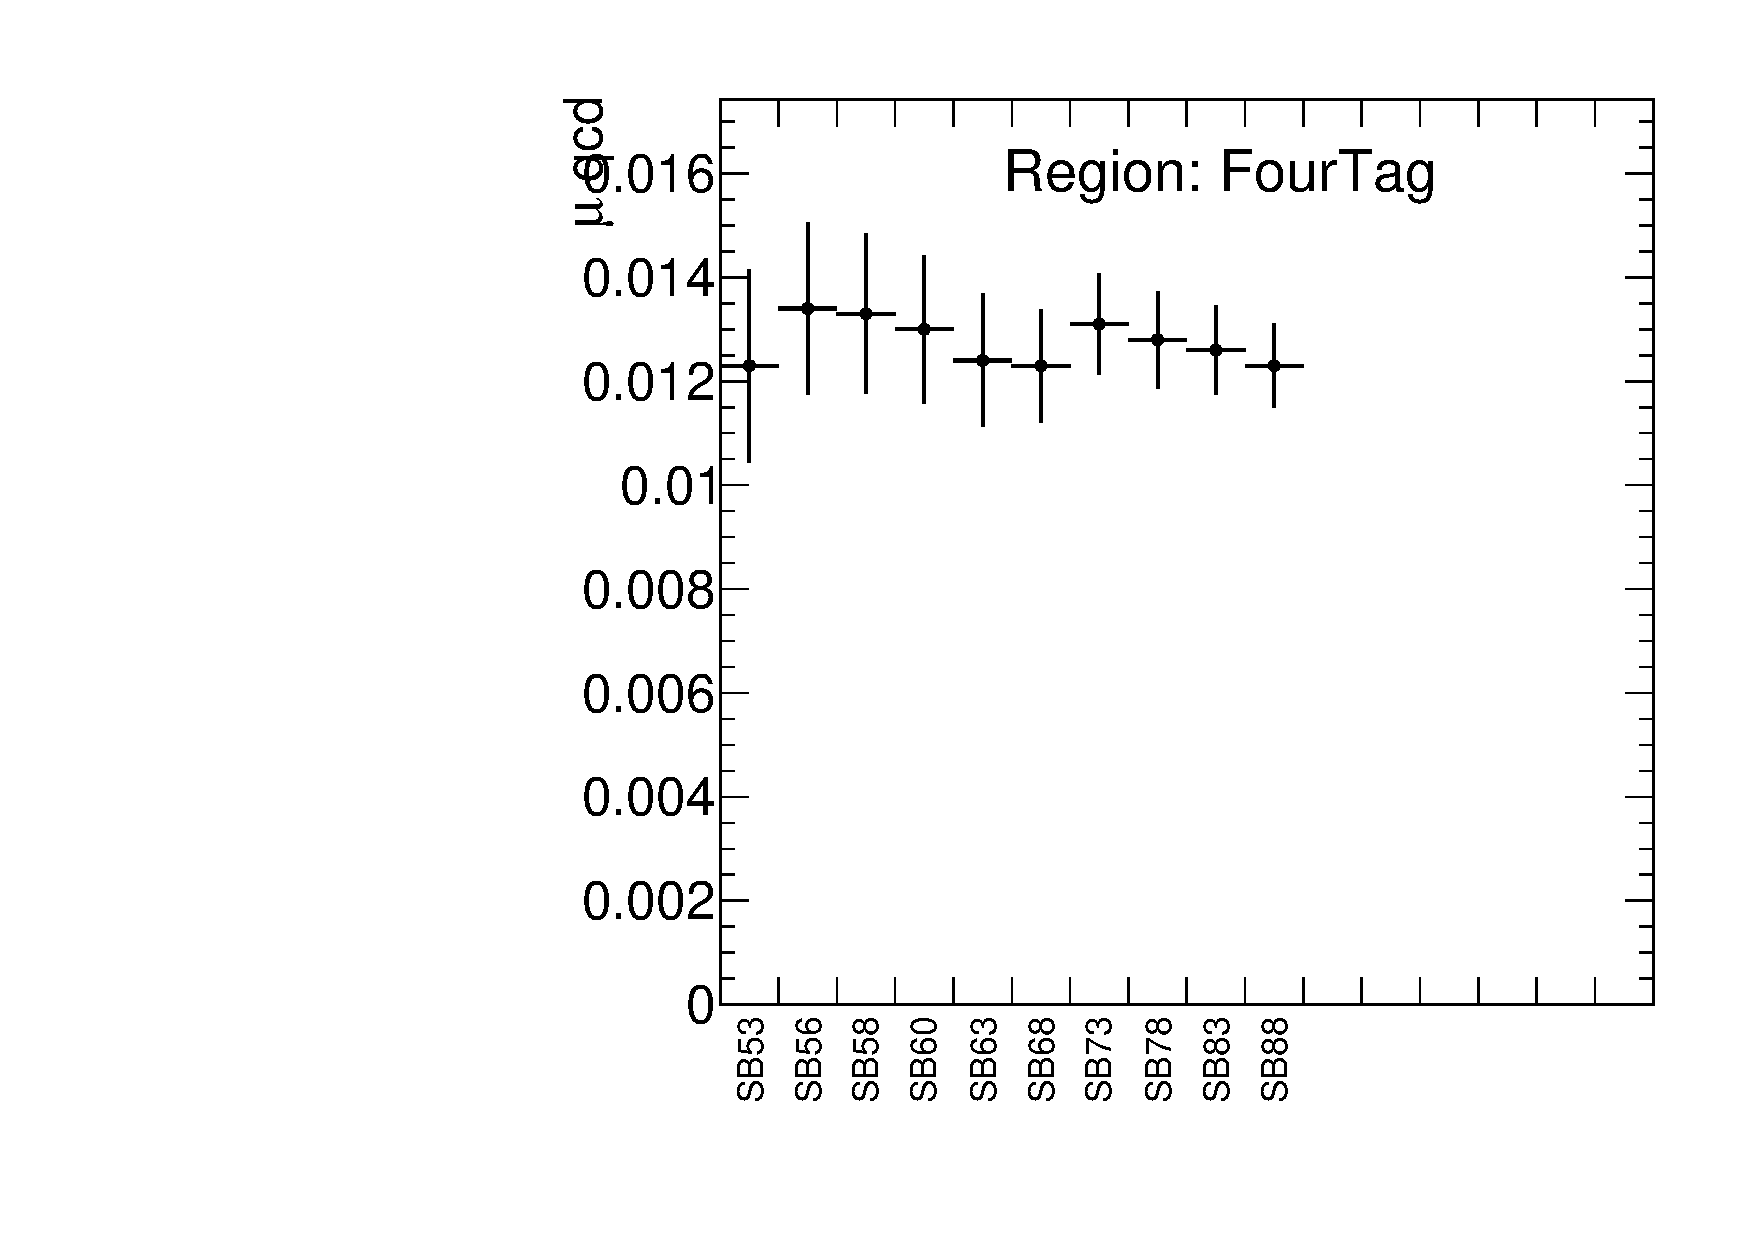
\includegraphics[angle=270, width=0.3\textwidth]{./figures/boosted/Appendix_SB/FourTag_muqcdSB.pdf}
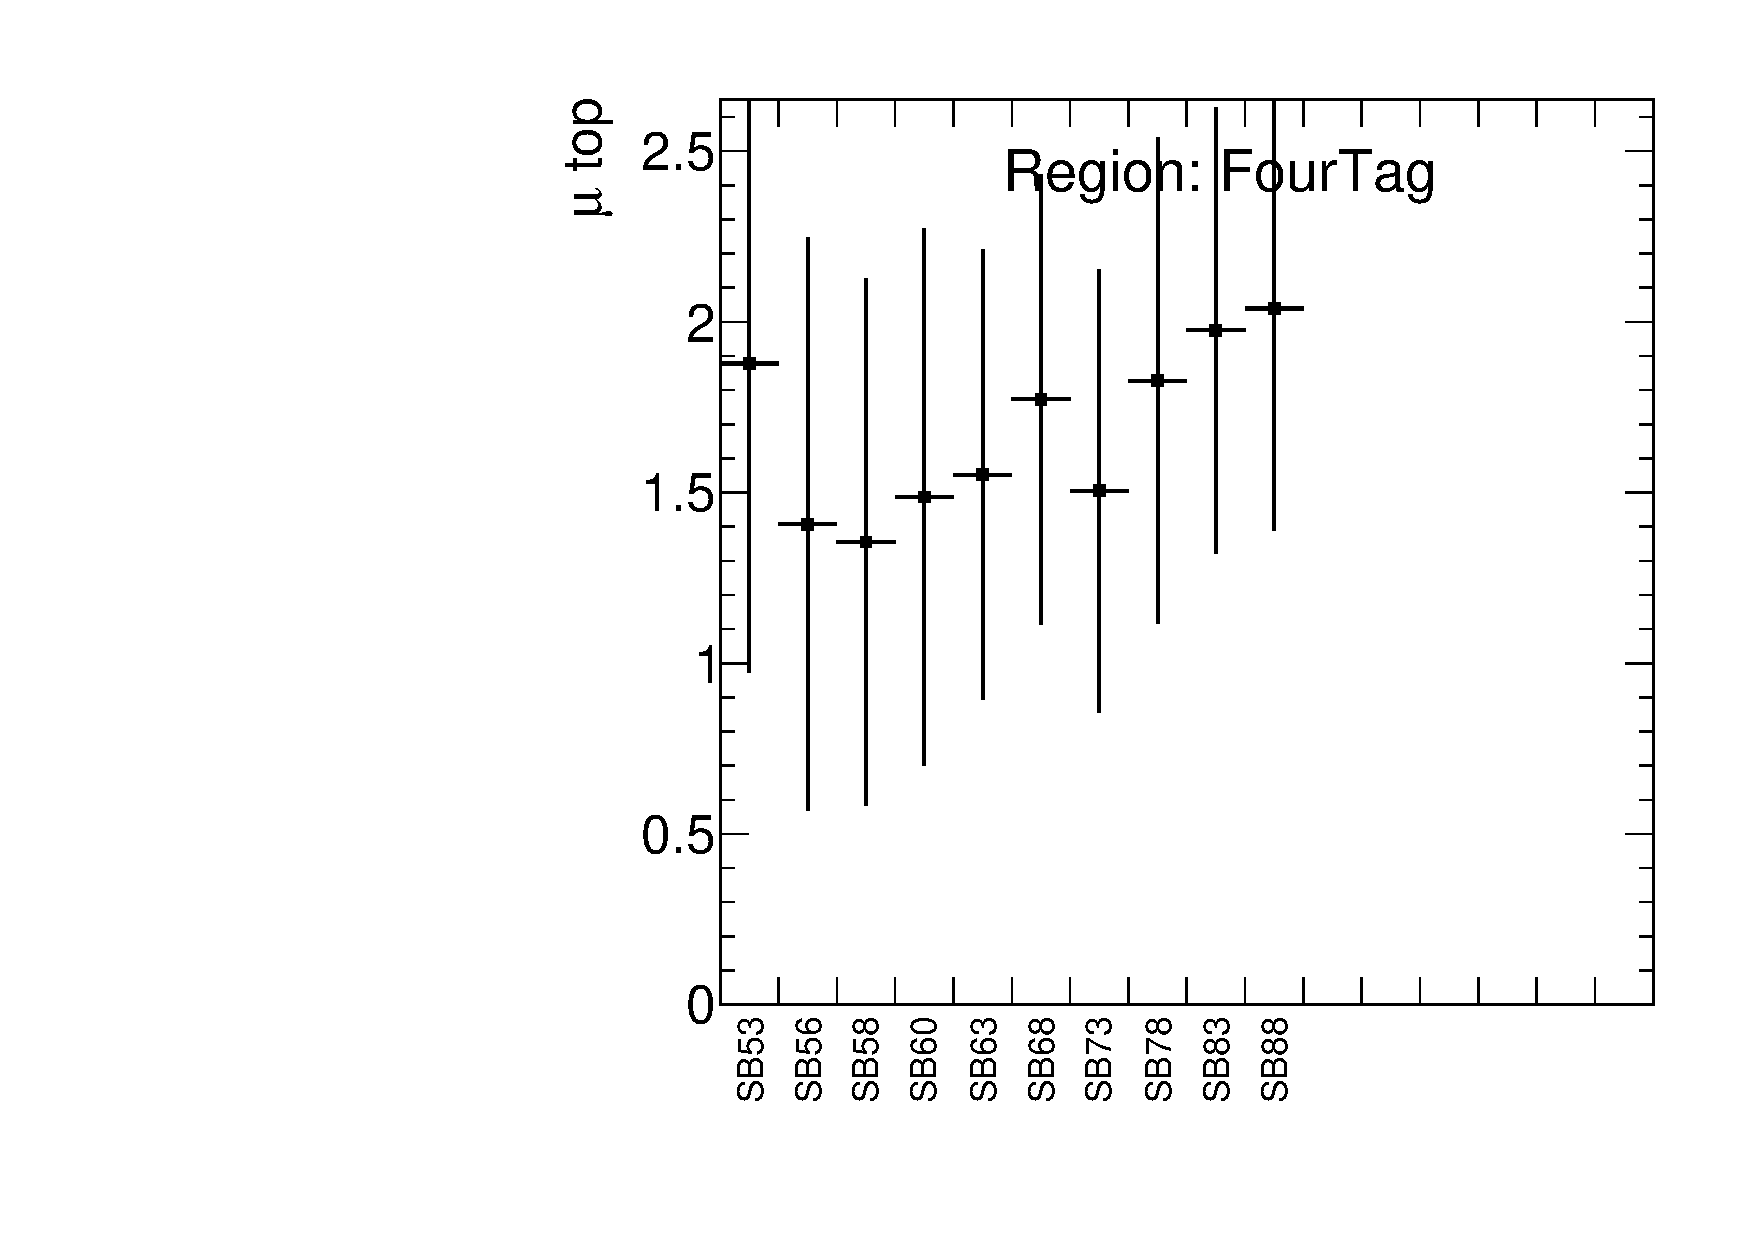
\includegraphics[angle=270, width=0.3\textwidth]{./figures/boosted/Appendix_SB/FourTag_mutopSB.pdf}
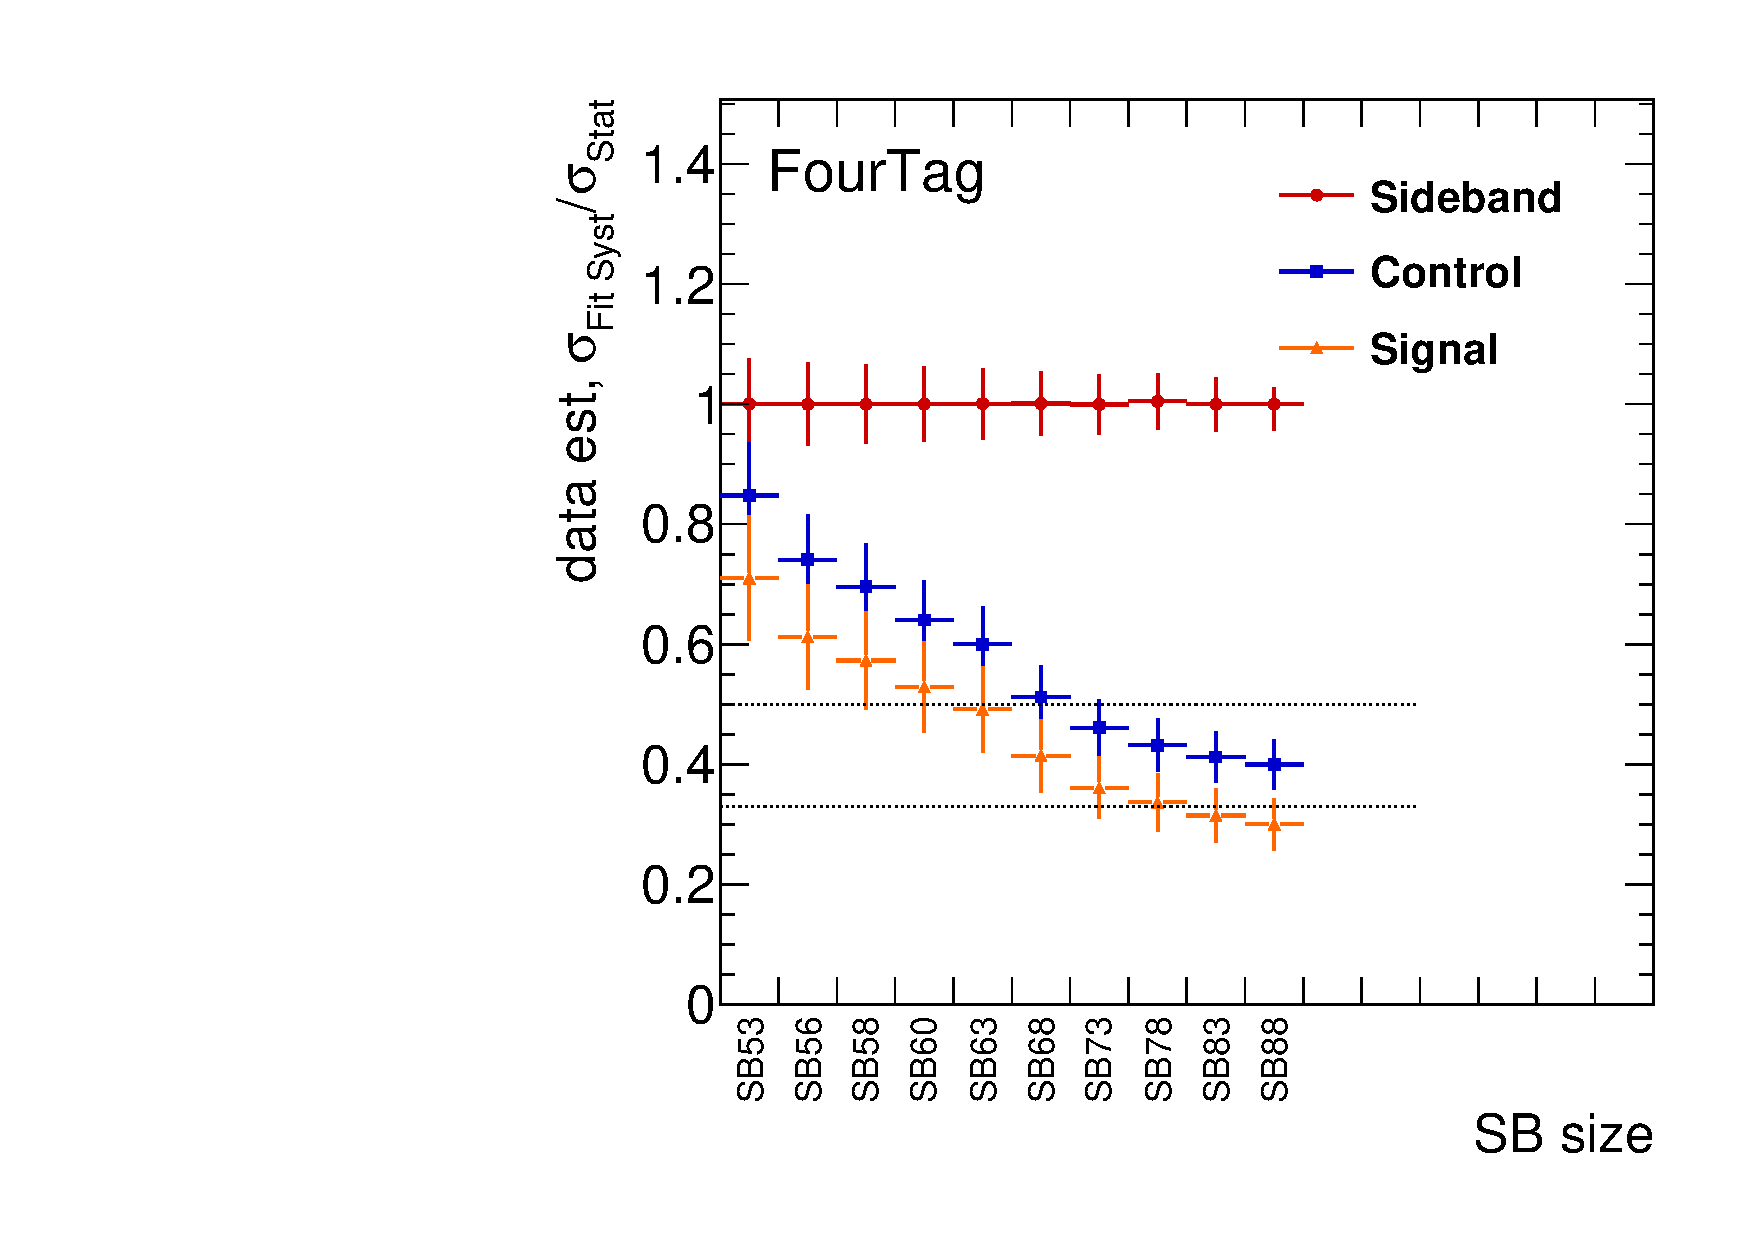
\includegraphics[angle=270, width=0.33\textwidth]{./figures/boosted/Appendix_SB/data_est_FourTag_sigma_compareSB.pdf}\\
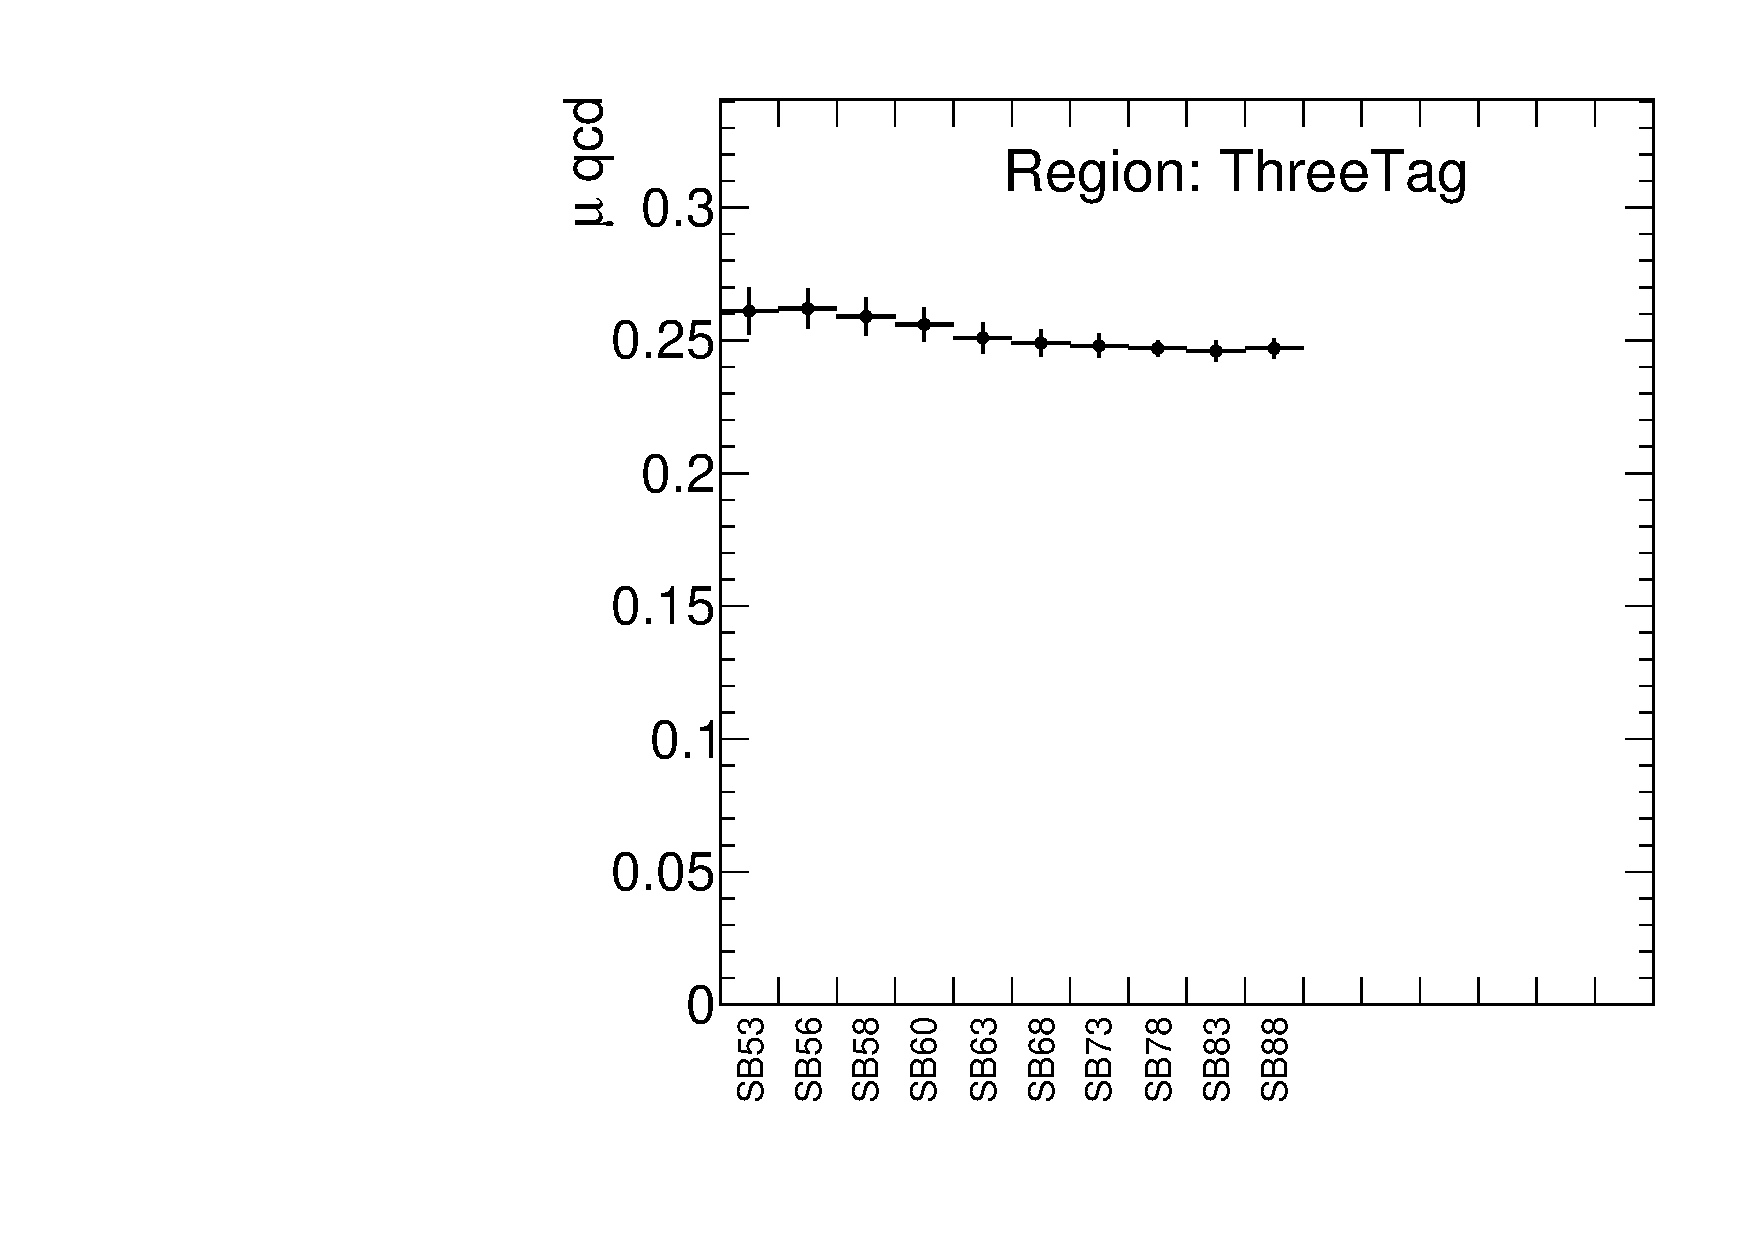
\includegraphics[angle=270, width=0.3\textwidth]{./figures/boosted/Appendix_SB/ThreeTag_muqcdSB.pdf}
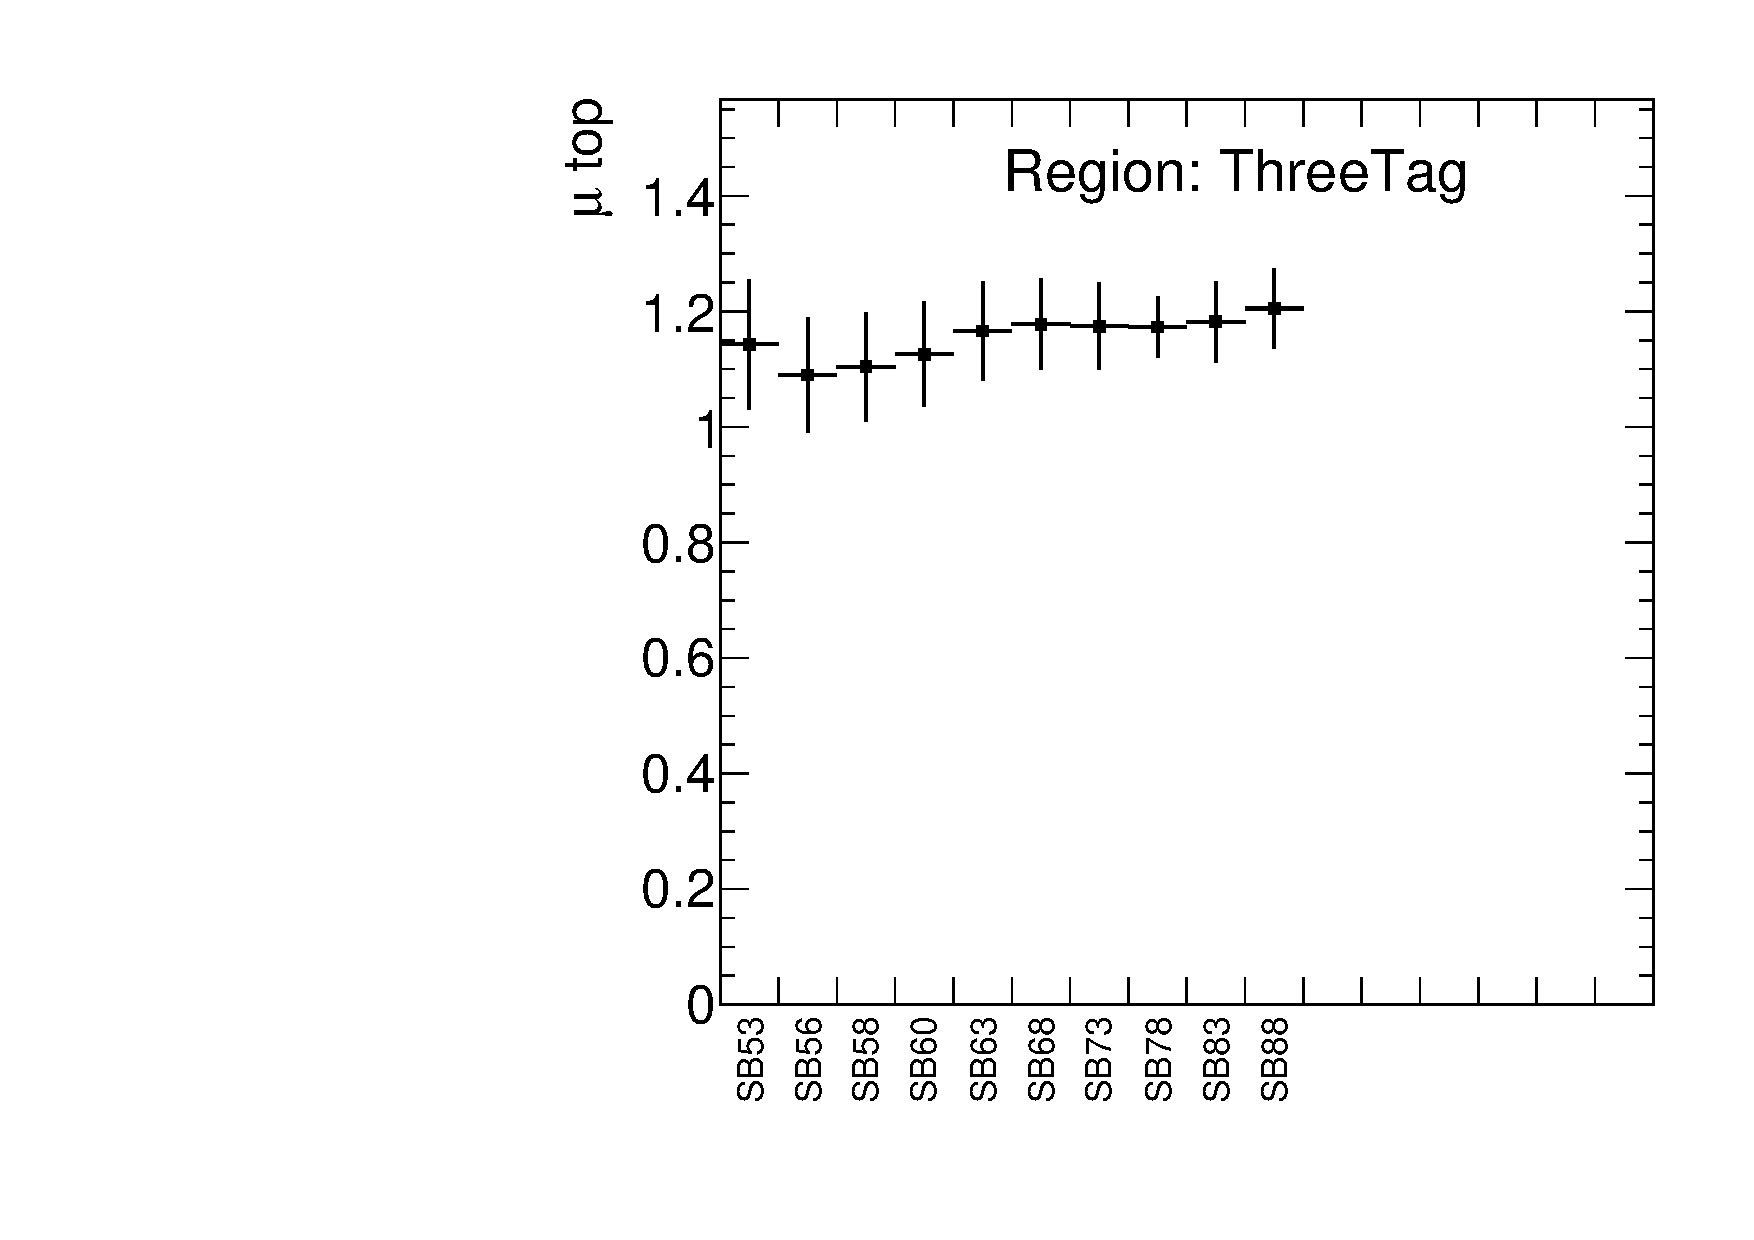
\includegraphics[angle=270, width=0.3\textwidth]{./figures/boosted/Appendix_SB/ThreeTag_mutopSB.pdf}
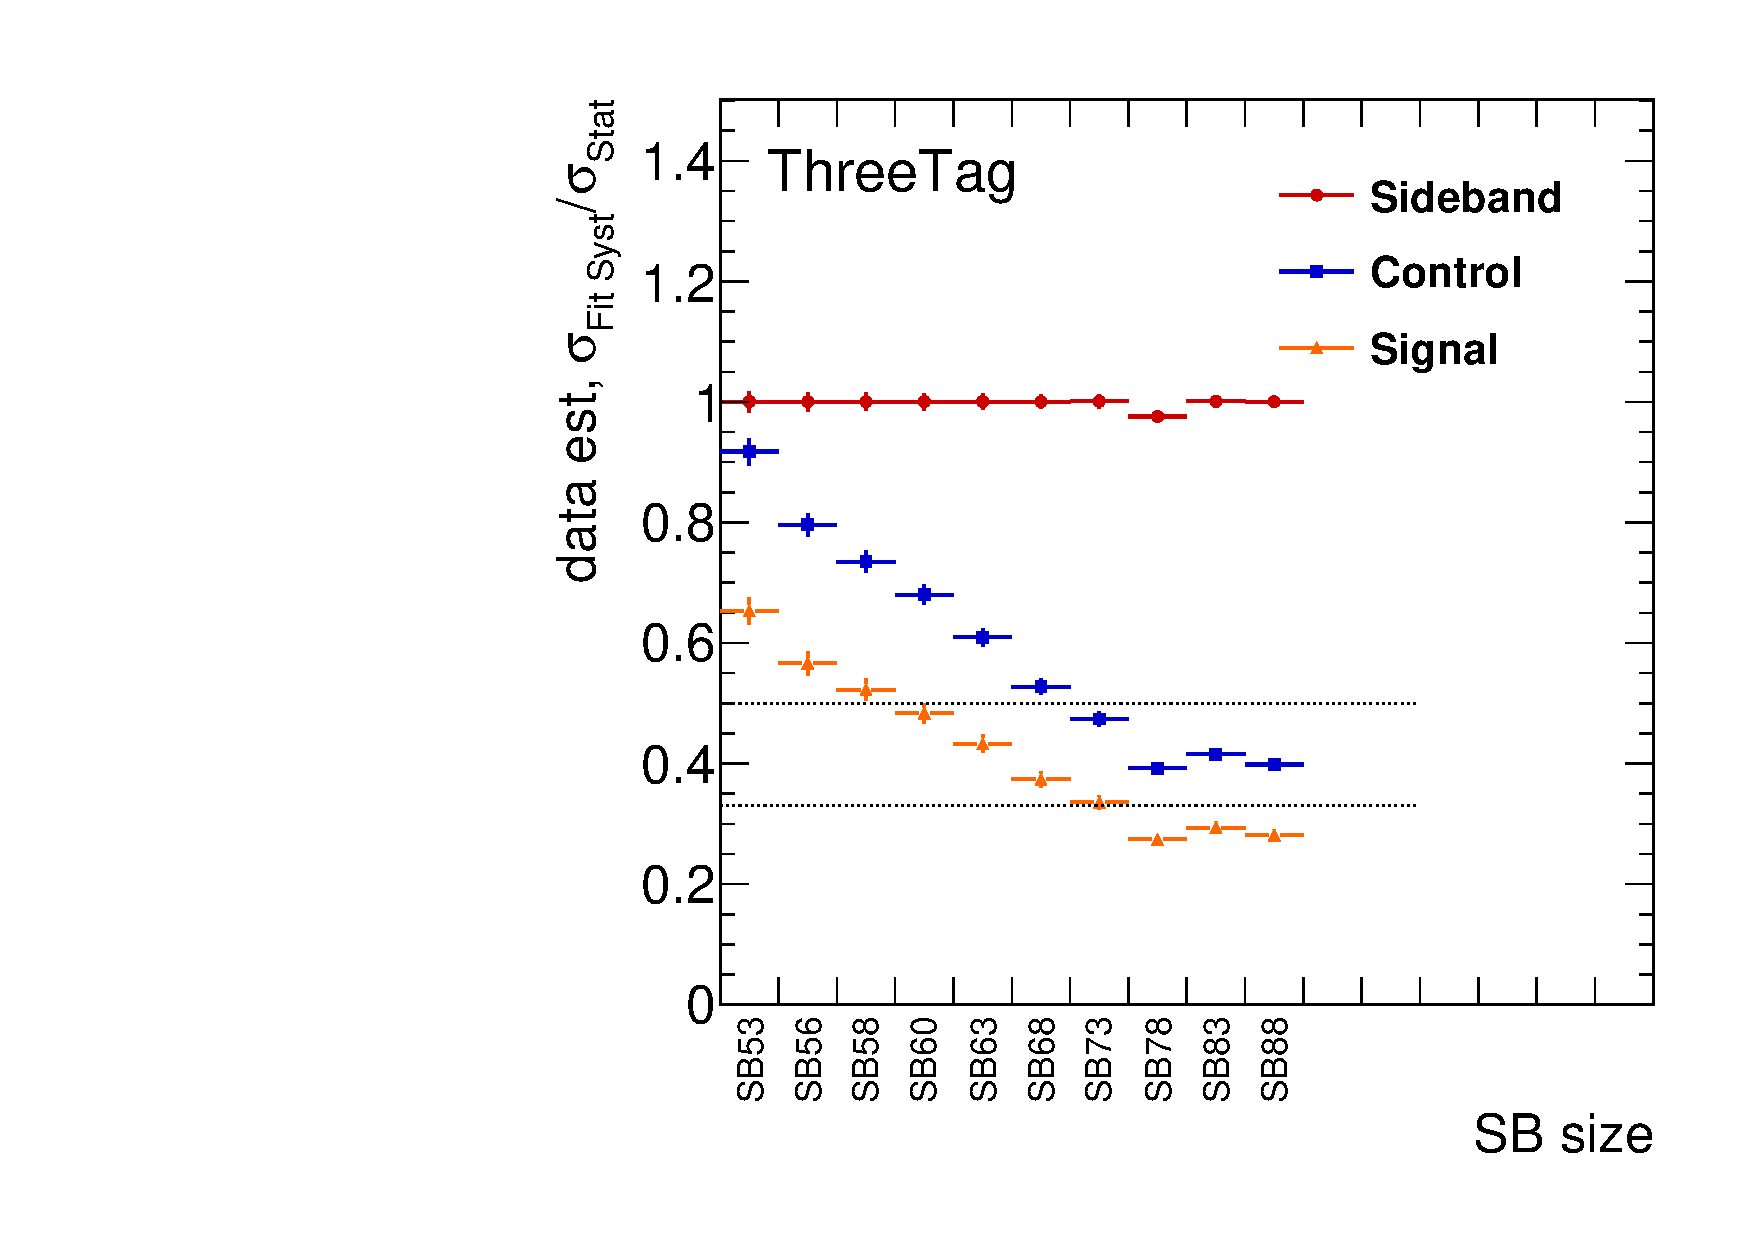
\includegraphics[angle=270, width=0.33\textwidth]{./figures/boosted/Appendix_SB/data_est_ThreeTag_sigma_compareSB.pdf}\\
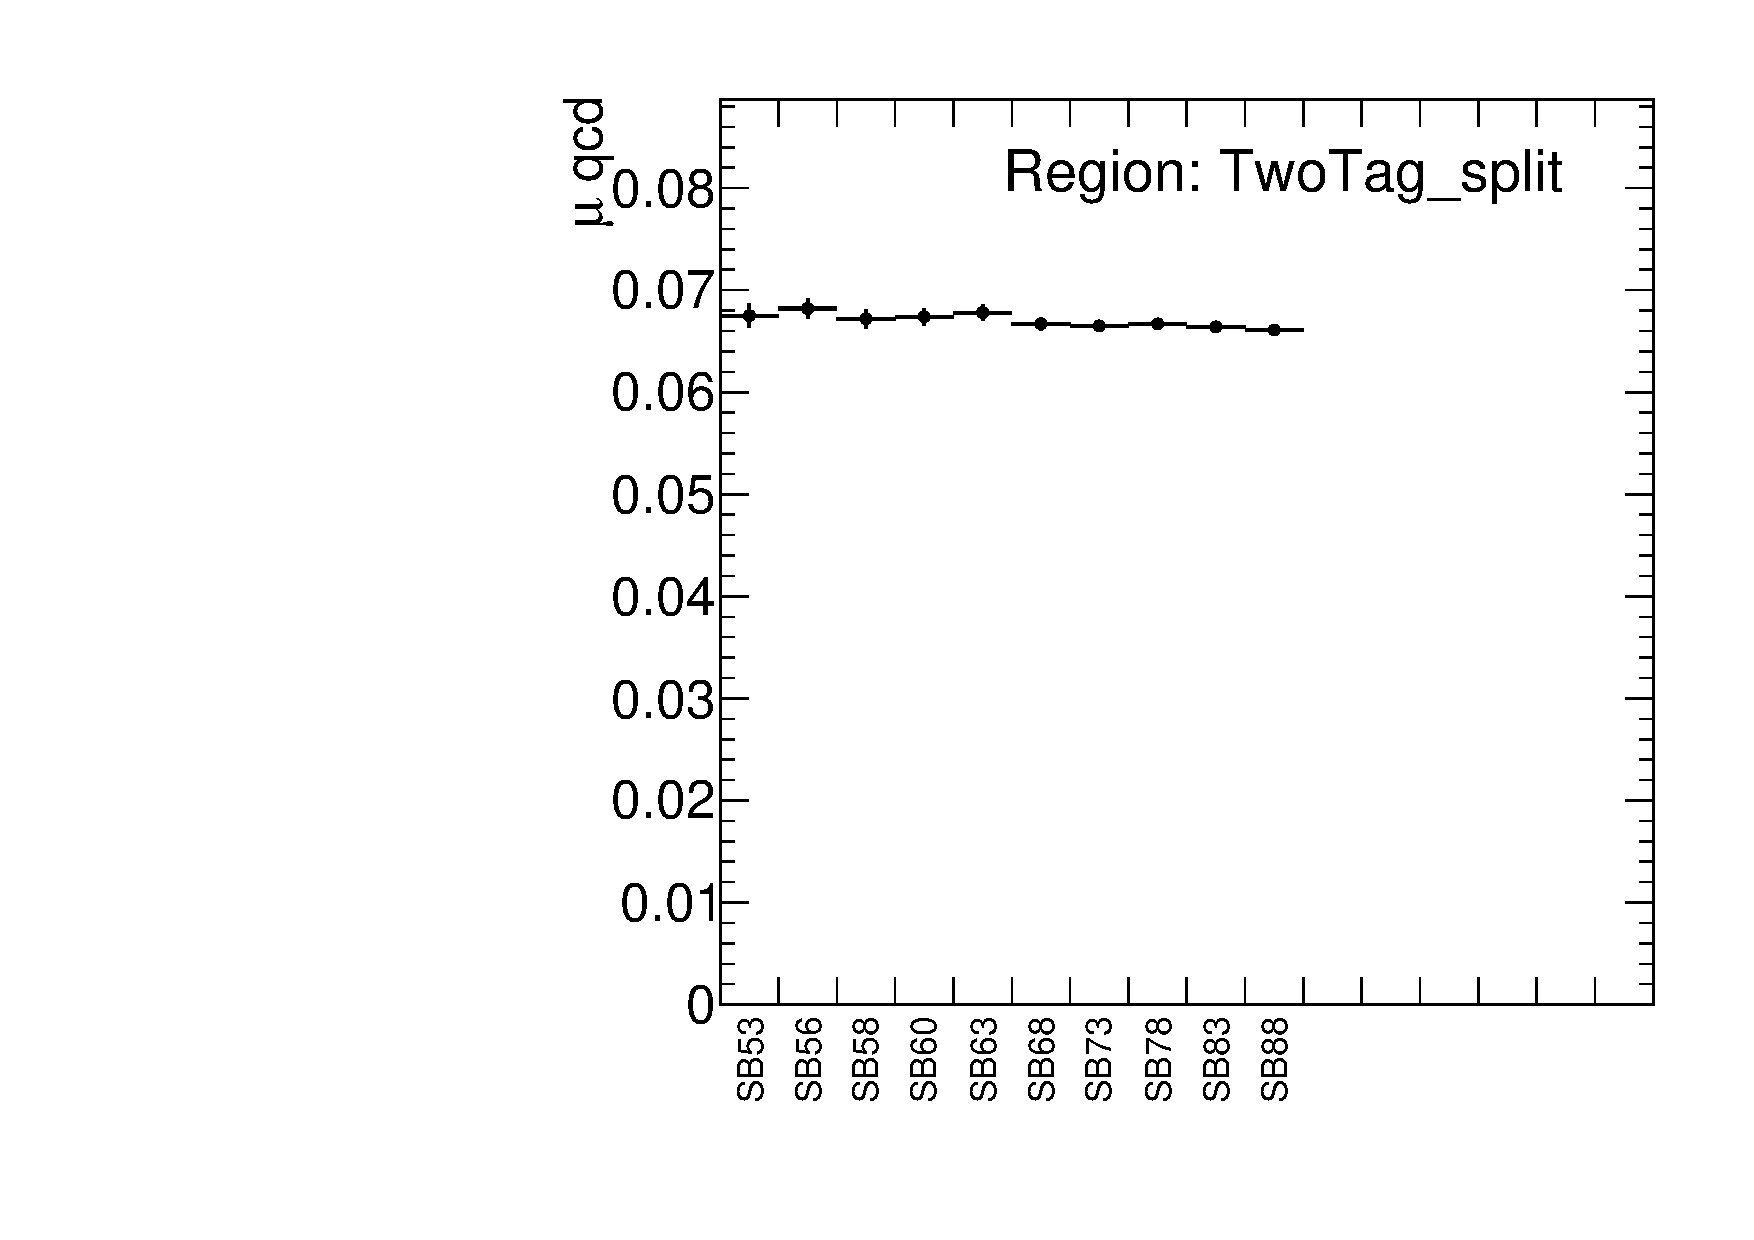
\includegraphics[angle=270, width=0.3\textwidth]{./figures/boosted/Appendix_SB/TwoTag_split_muqcdSB.pdf}
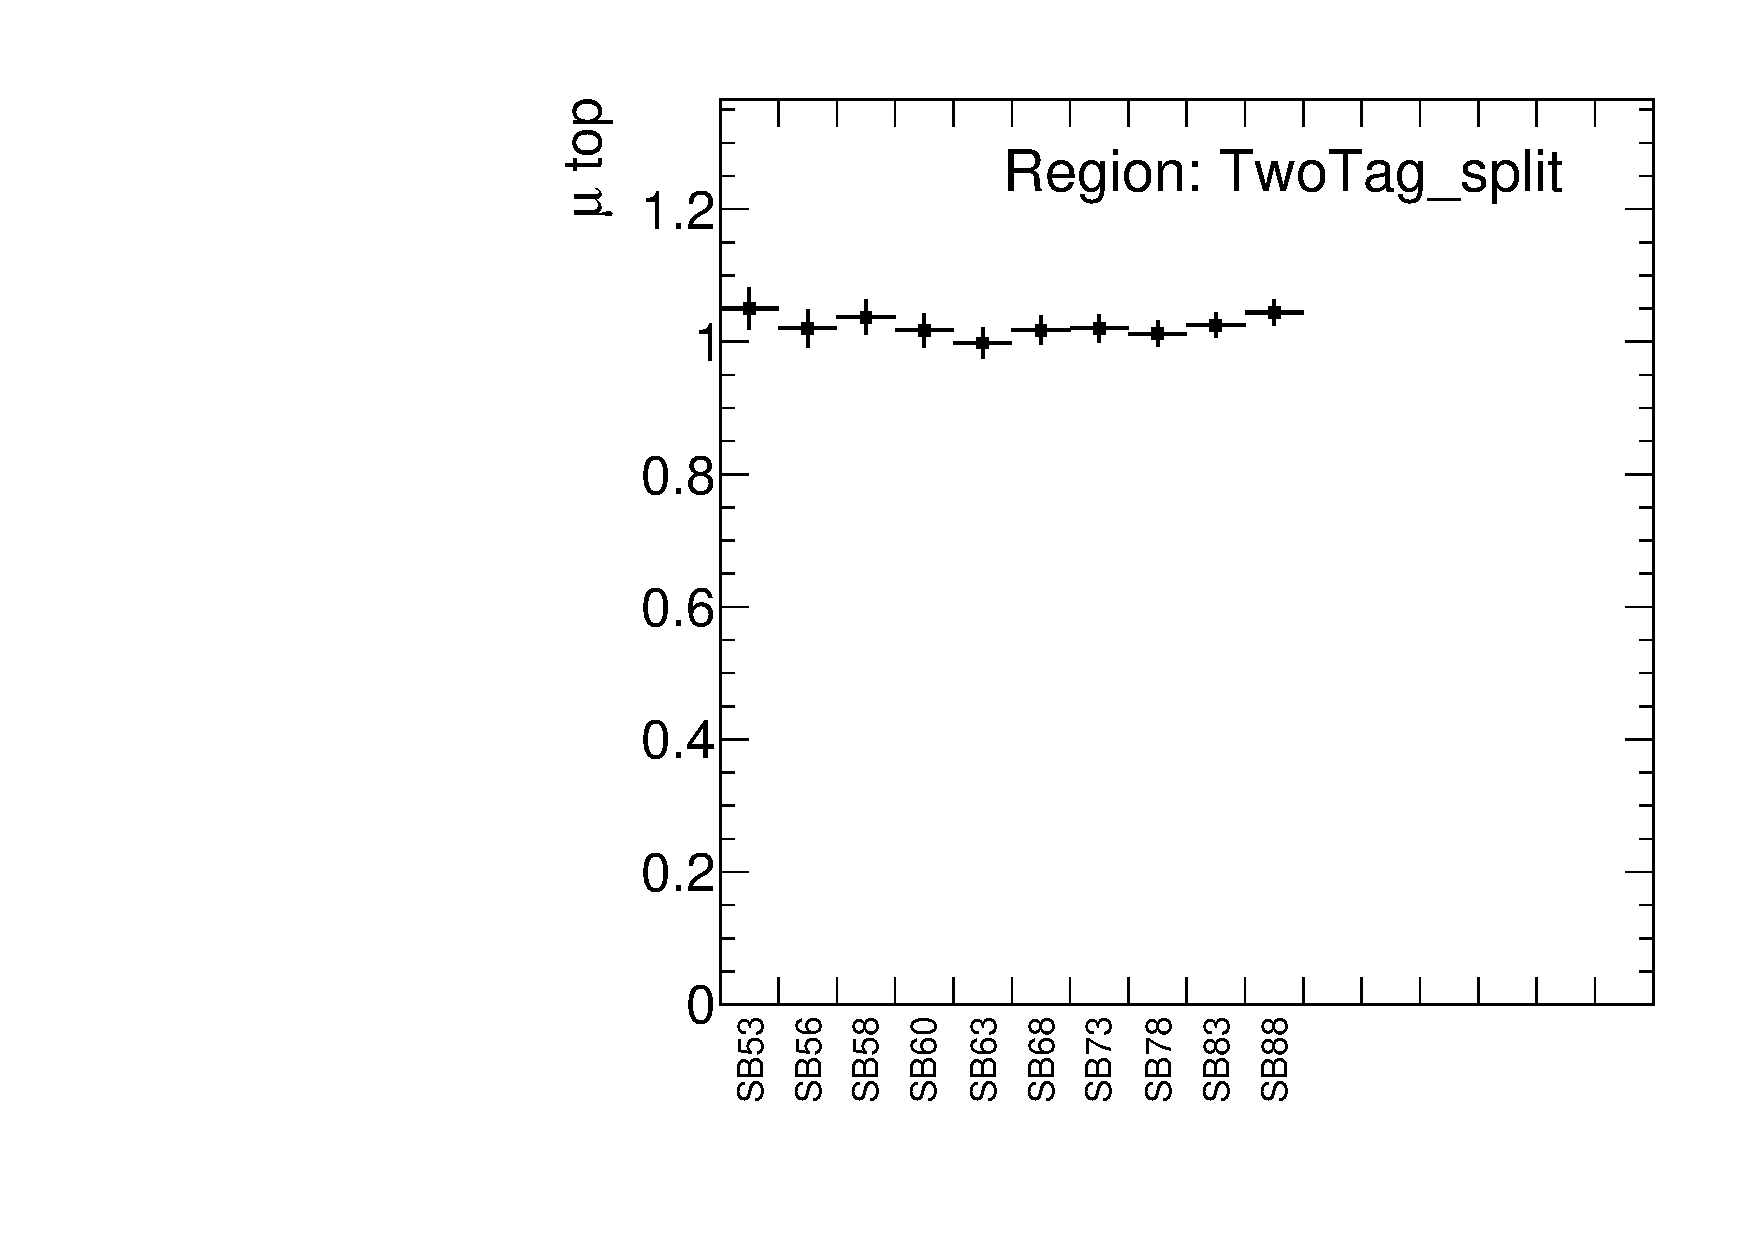
\includegraphics[angle=270, width=0.3\textwidth]{./figures/boosted/Appendix_SB/TwoTag_split_mutopSB.pdf}
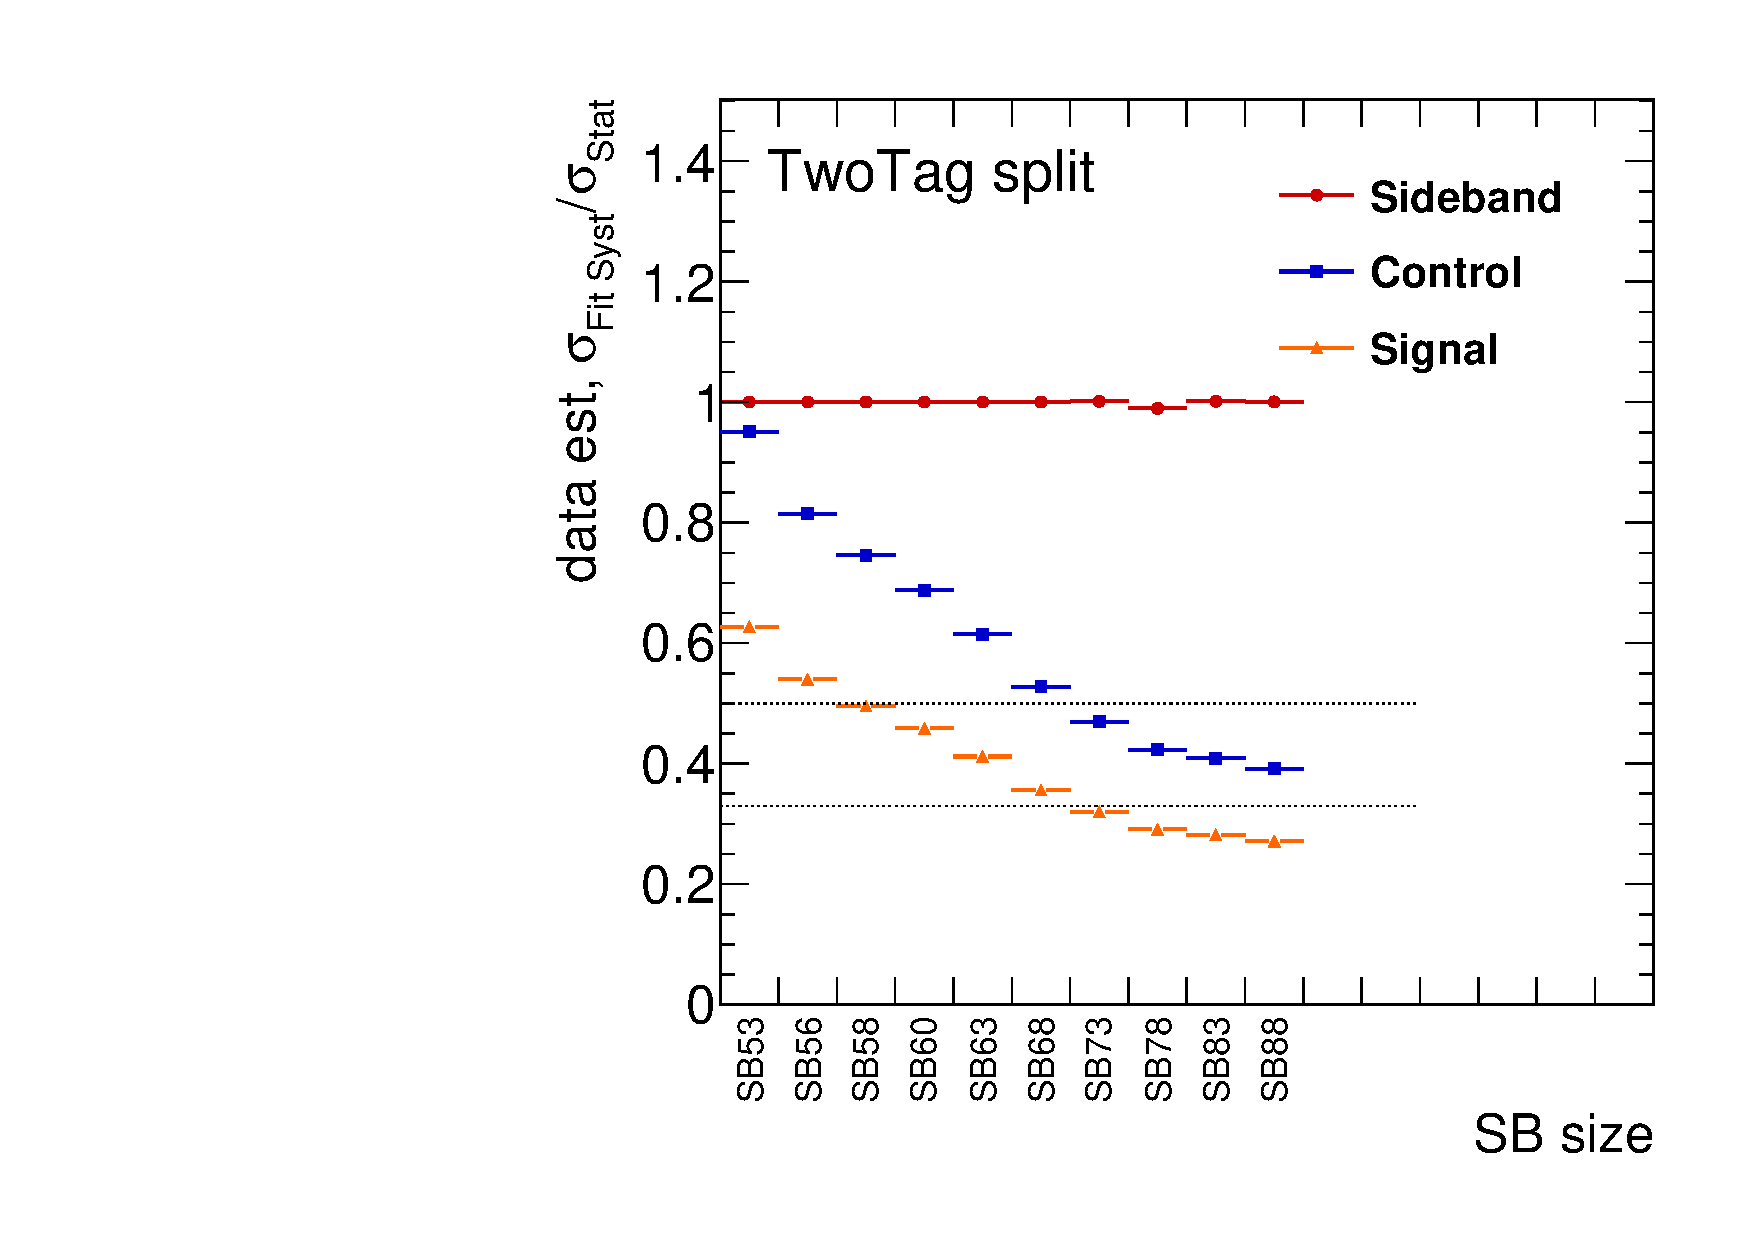
\includegraphics[angle=270, width=0.33\textwidth]{./figures/boosted/Appendix_SB/data_est_TwoTag_split_sigma_compareSB.pdf}
  \caption{Fit parameters for $\mu_{\text{qcd}}$ (left), $\alpha_{t\bar{t}}$ (middle), and ratio of fit uncertainty and stat uncertainty as a functioin of different Sideband values (right) , for 4$b$ (top) 3$b$ (middle) and 2$b$s (bottom). The x-axis indicates different values of SB $R_{hh}^{\text{high}}$ cuts.}
  \label{fig:app-sb-muqcd-diffSB}
\end{center}
\end{figure*}


\paragraph{} A similar test can be done on different Sideband Region shifts. This is shown in Figure~\ref{fig:app-sb-muqcd-diffSBshift}. Based on the choice that for the signal region predictions, the fit uncertainty should be around half of the statistical uncertainty, the Sideband center shift is chosen to be 10 \GeV.

\begin{figure*}[htbp!]
\begin{center}
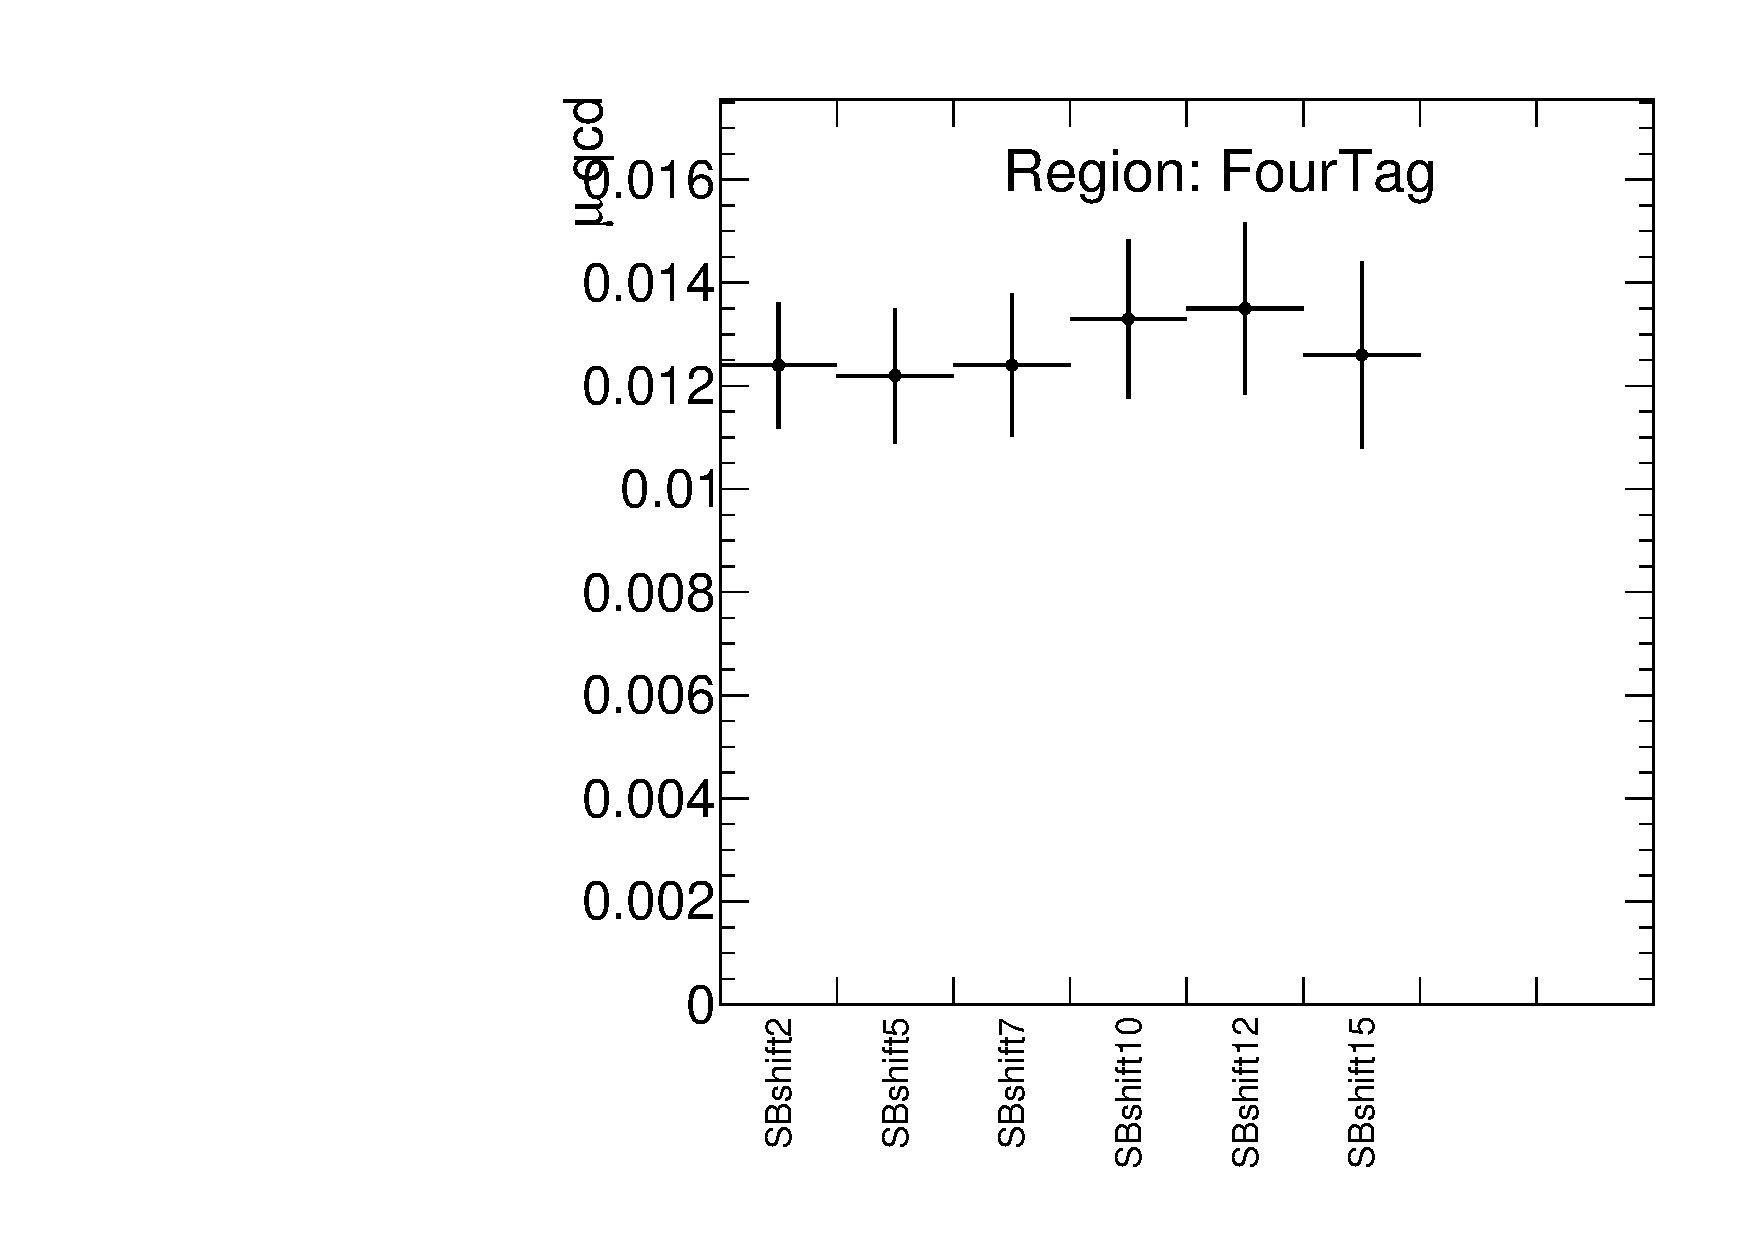
\includegraphics[angle=270, width=0.3\textwidth]{./figures/boosted/Appendix_SB/FourTag_muqcdSBshift.pdf}
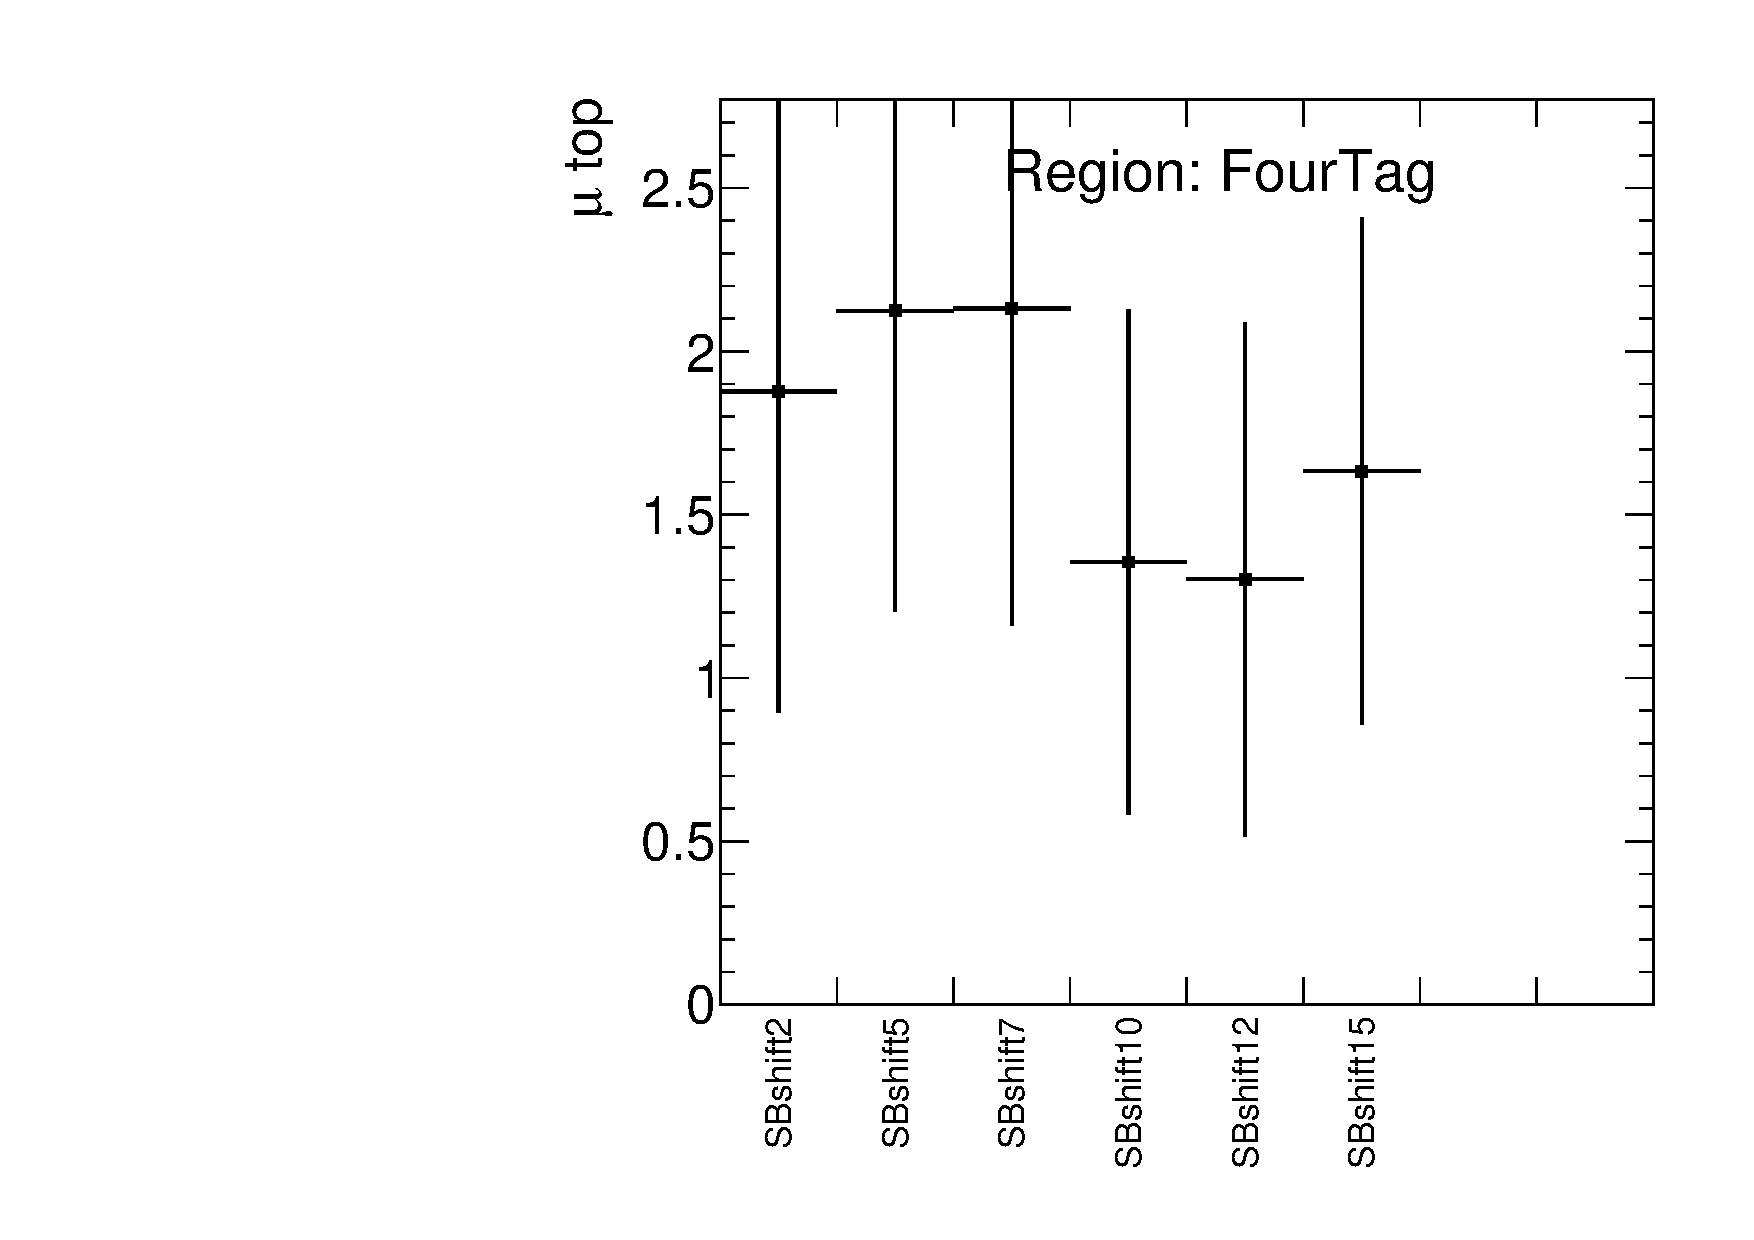
\includegraphics[angle=270, width=0.3\textwidth]{./figures/boosted/Appendix_SB/FourTag_mutopSBshift.pdf}
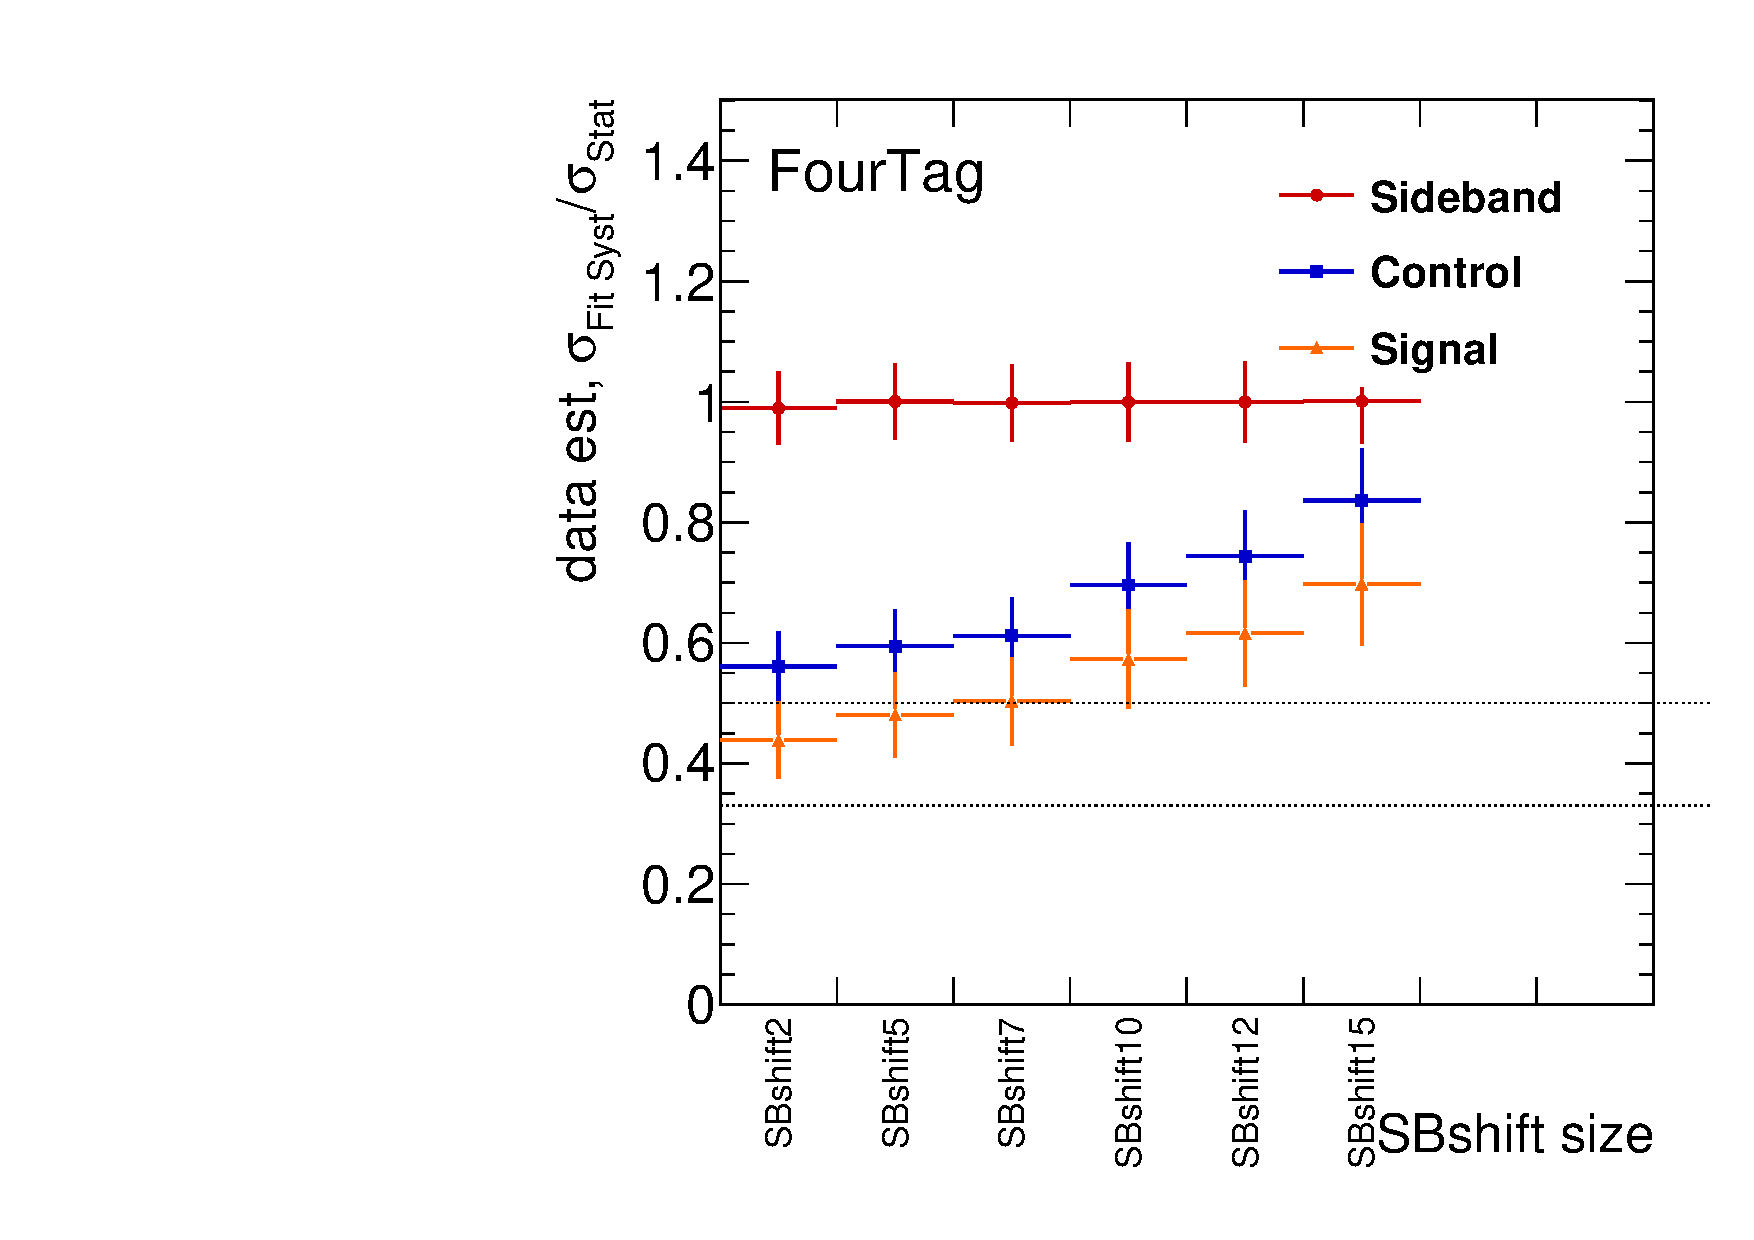
\includegraphics[angle=270, width=0.33\textwidth]{./figures/boosted/Appendix_SB/data_est_FourTag_sigma_compareSBshift.pdf}\\
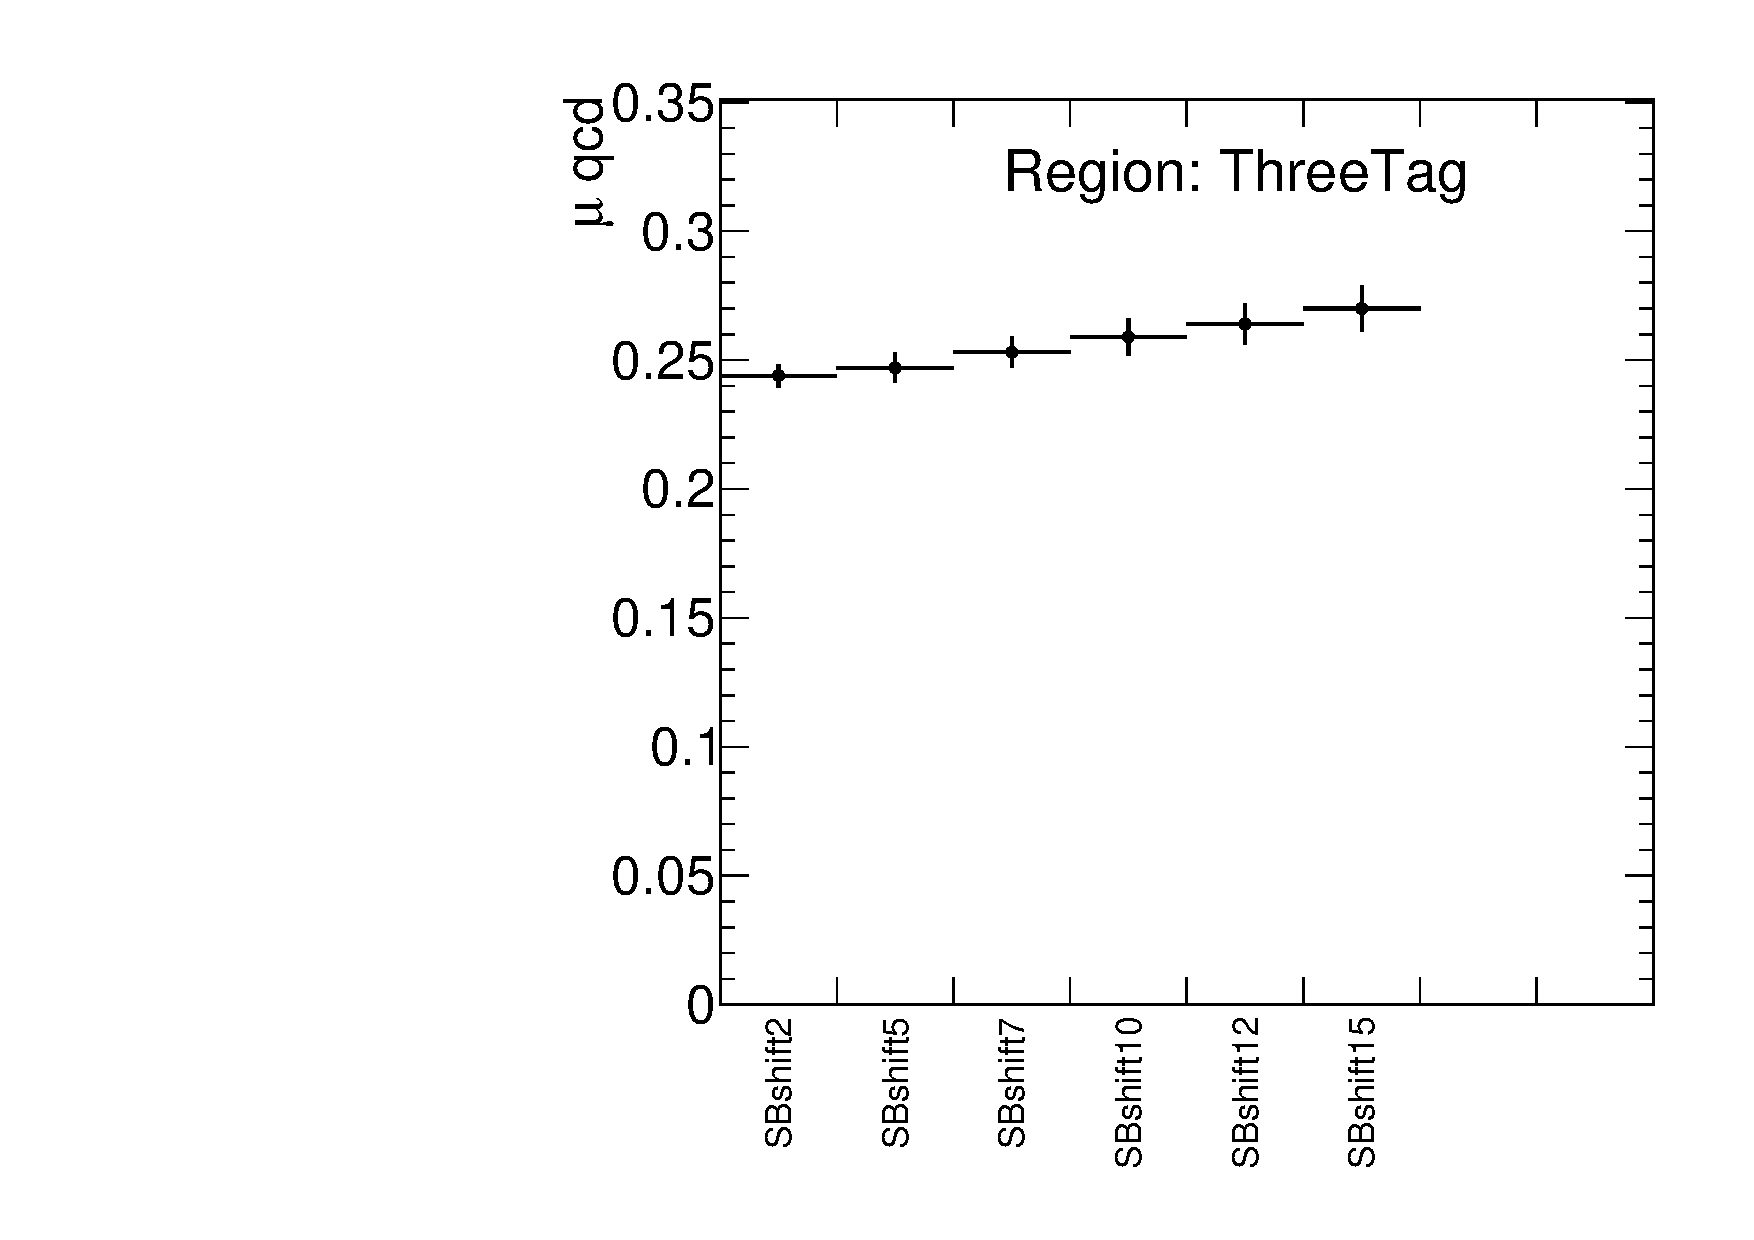
\includegraphics[angle=270, width=0.3\textwidth]{./figures/boosted/Appendix_SB/ThreeTag_muqcdSBshift.pdf}
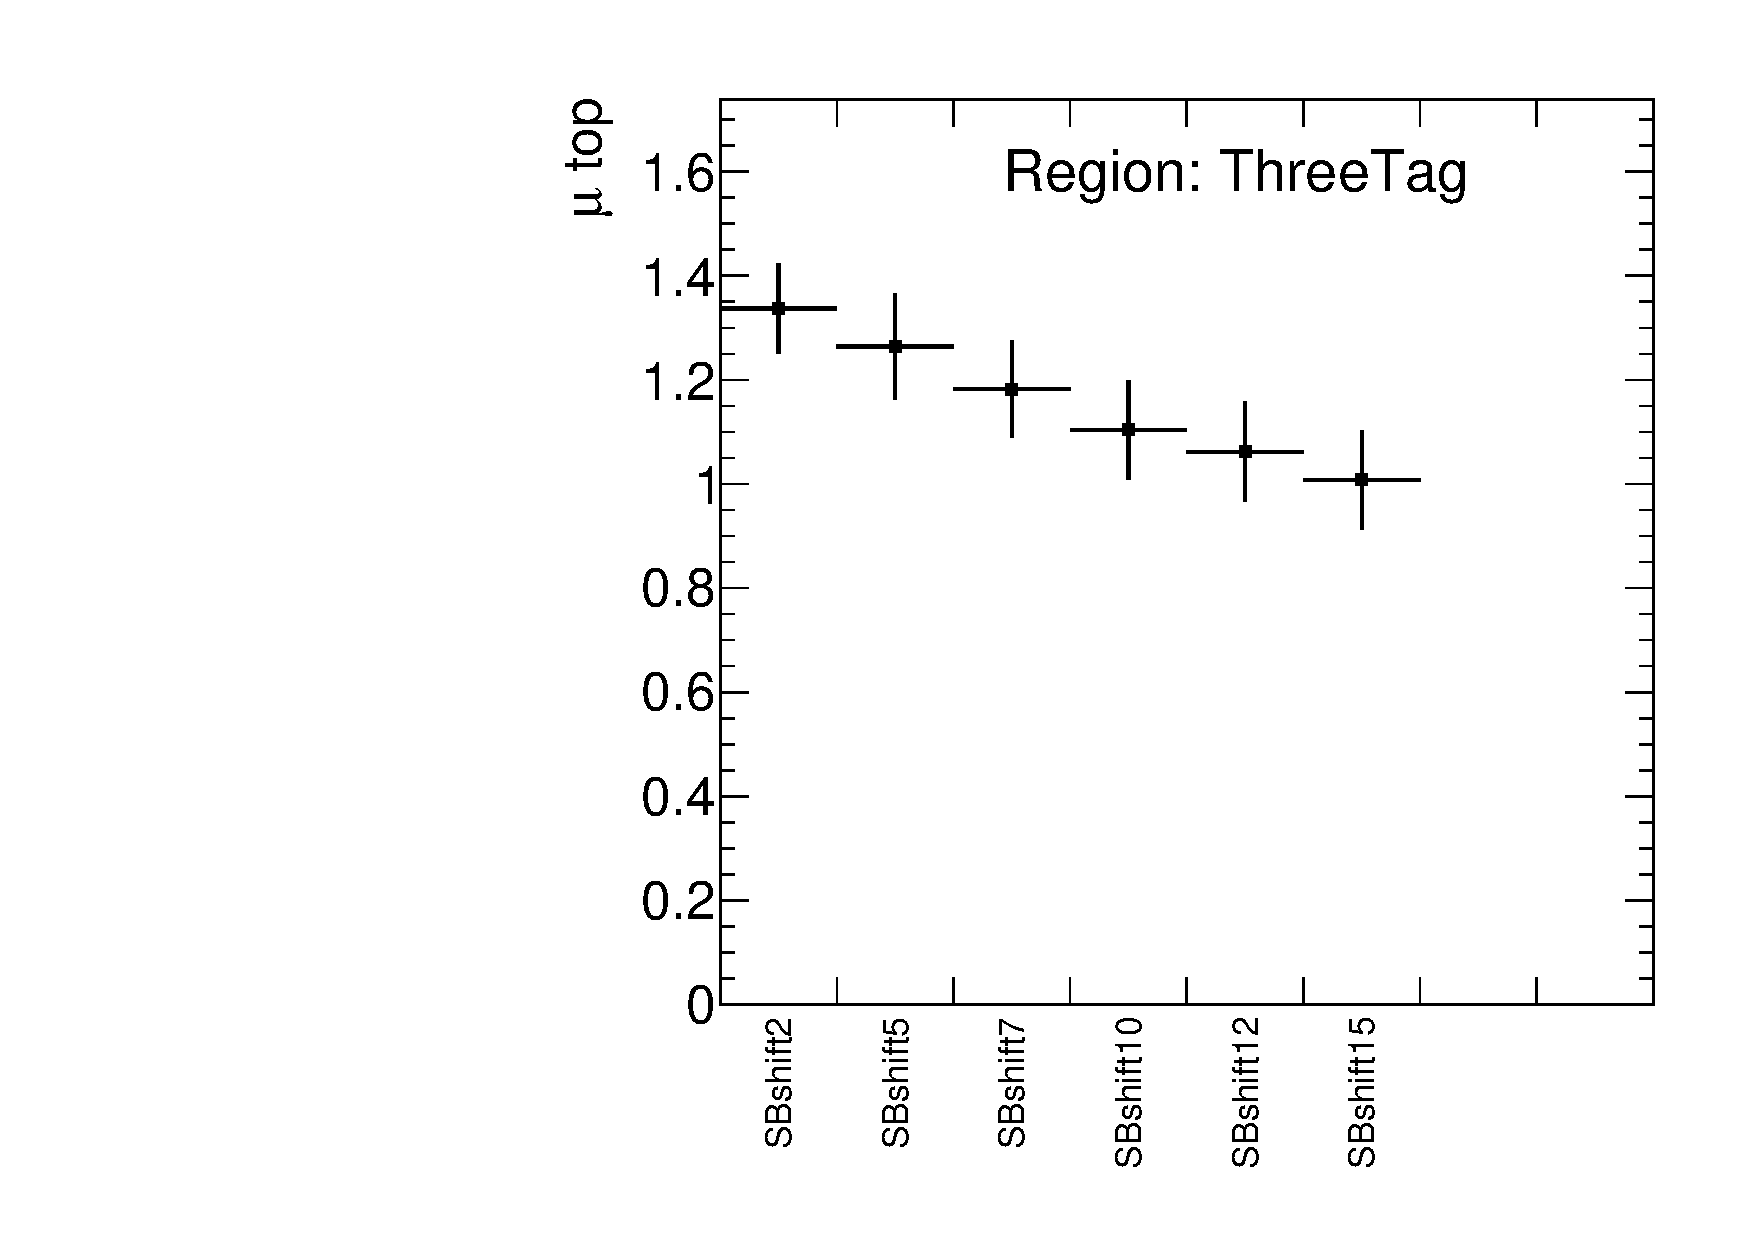
\includegraphics[angle=270, width=0.3\textwidth]{./figures/boosted/Appendix_SB/ThreeTag_mutopSBshift.pdf}
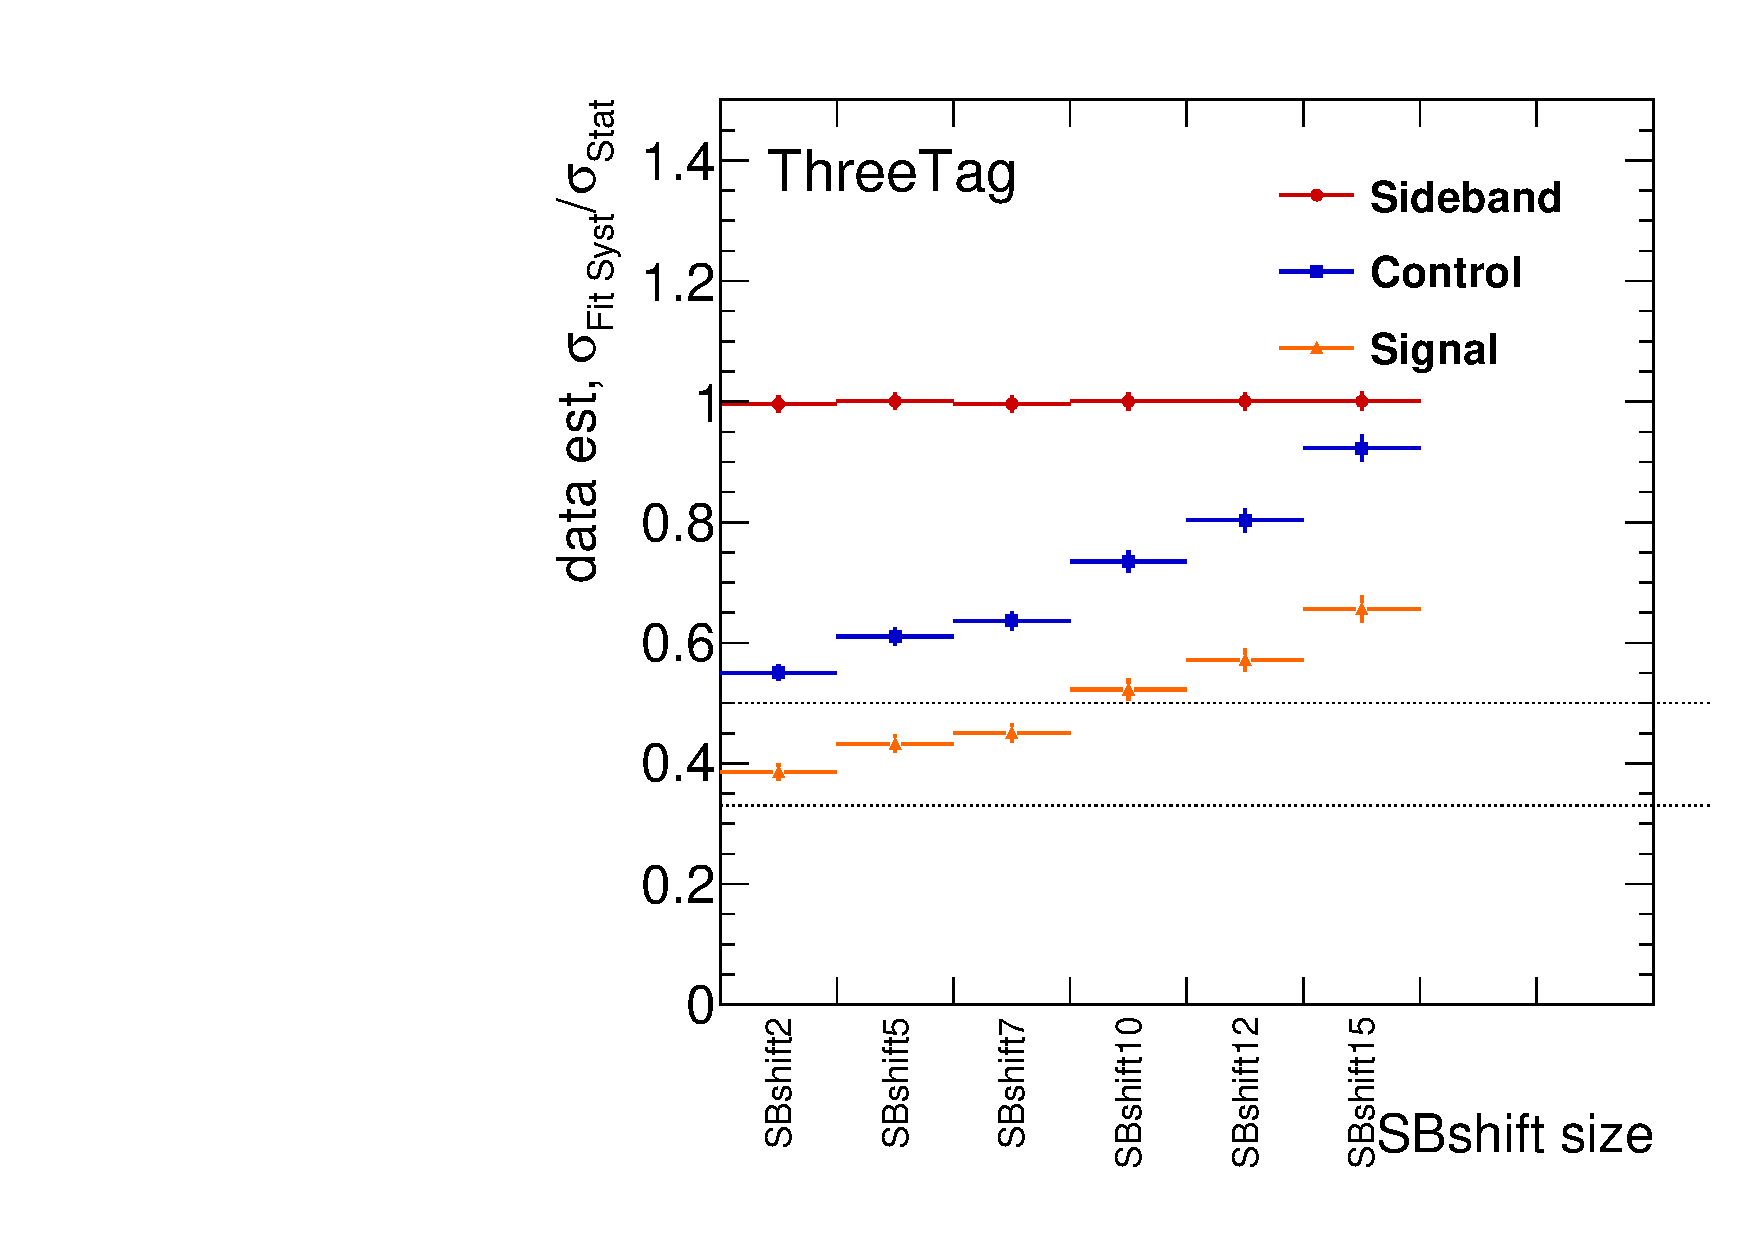
\includegraphics[angle=270, width=0.33\textwidth]{./figures/boosted/Appendix_SB/data_est_ThreeTag_sigma_compareSBshift.pdf}\\
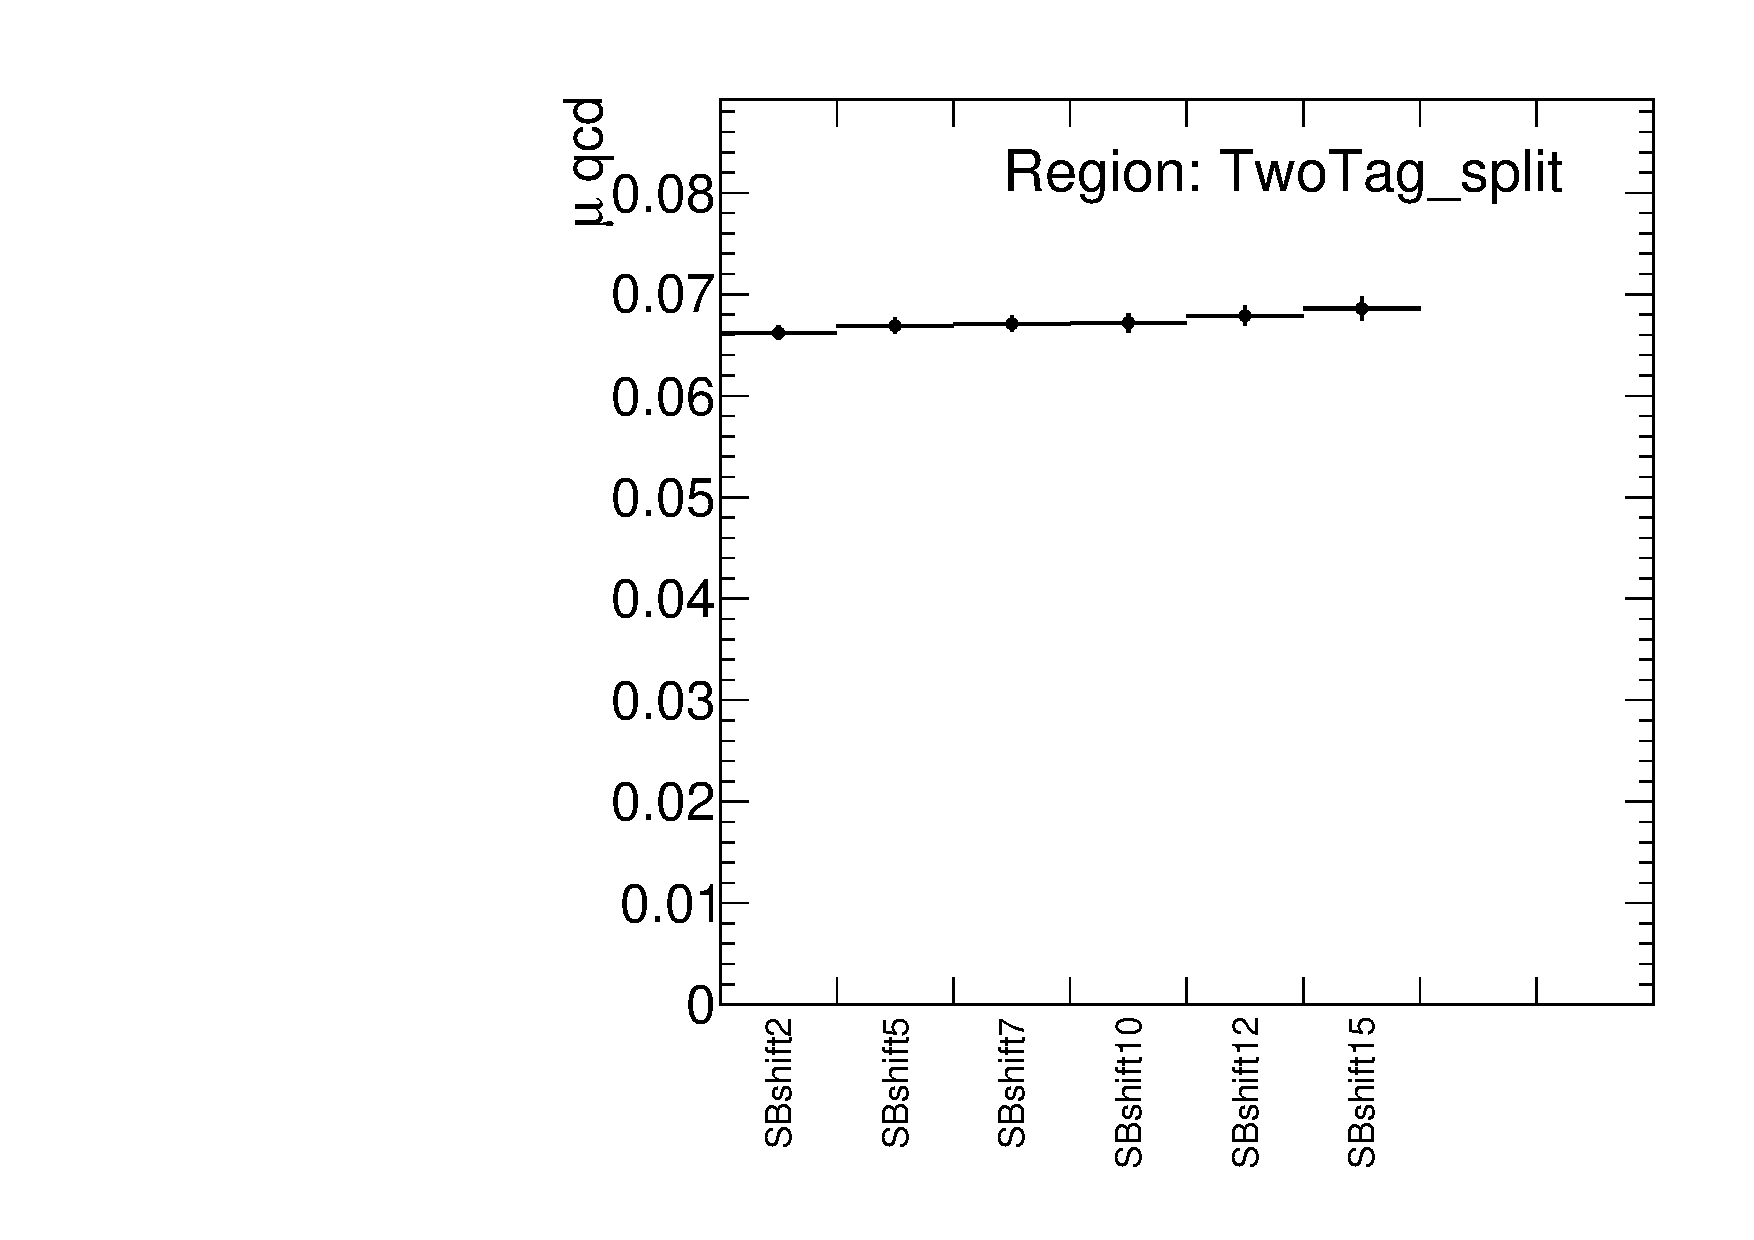
\includegraphics[angle=270, width=0.3\textwidth]{./figures/boosted/Appendix_SB/TwoTag_split_muqcdSBshift.pdf}
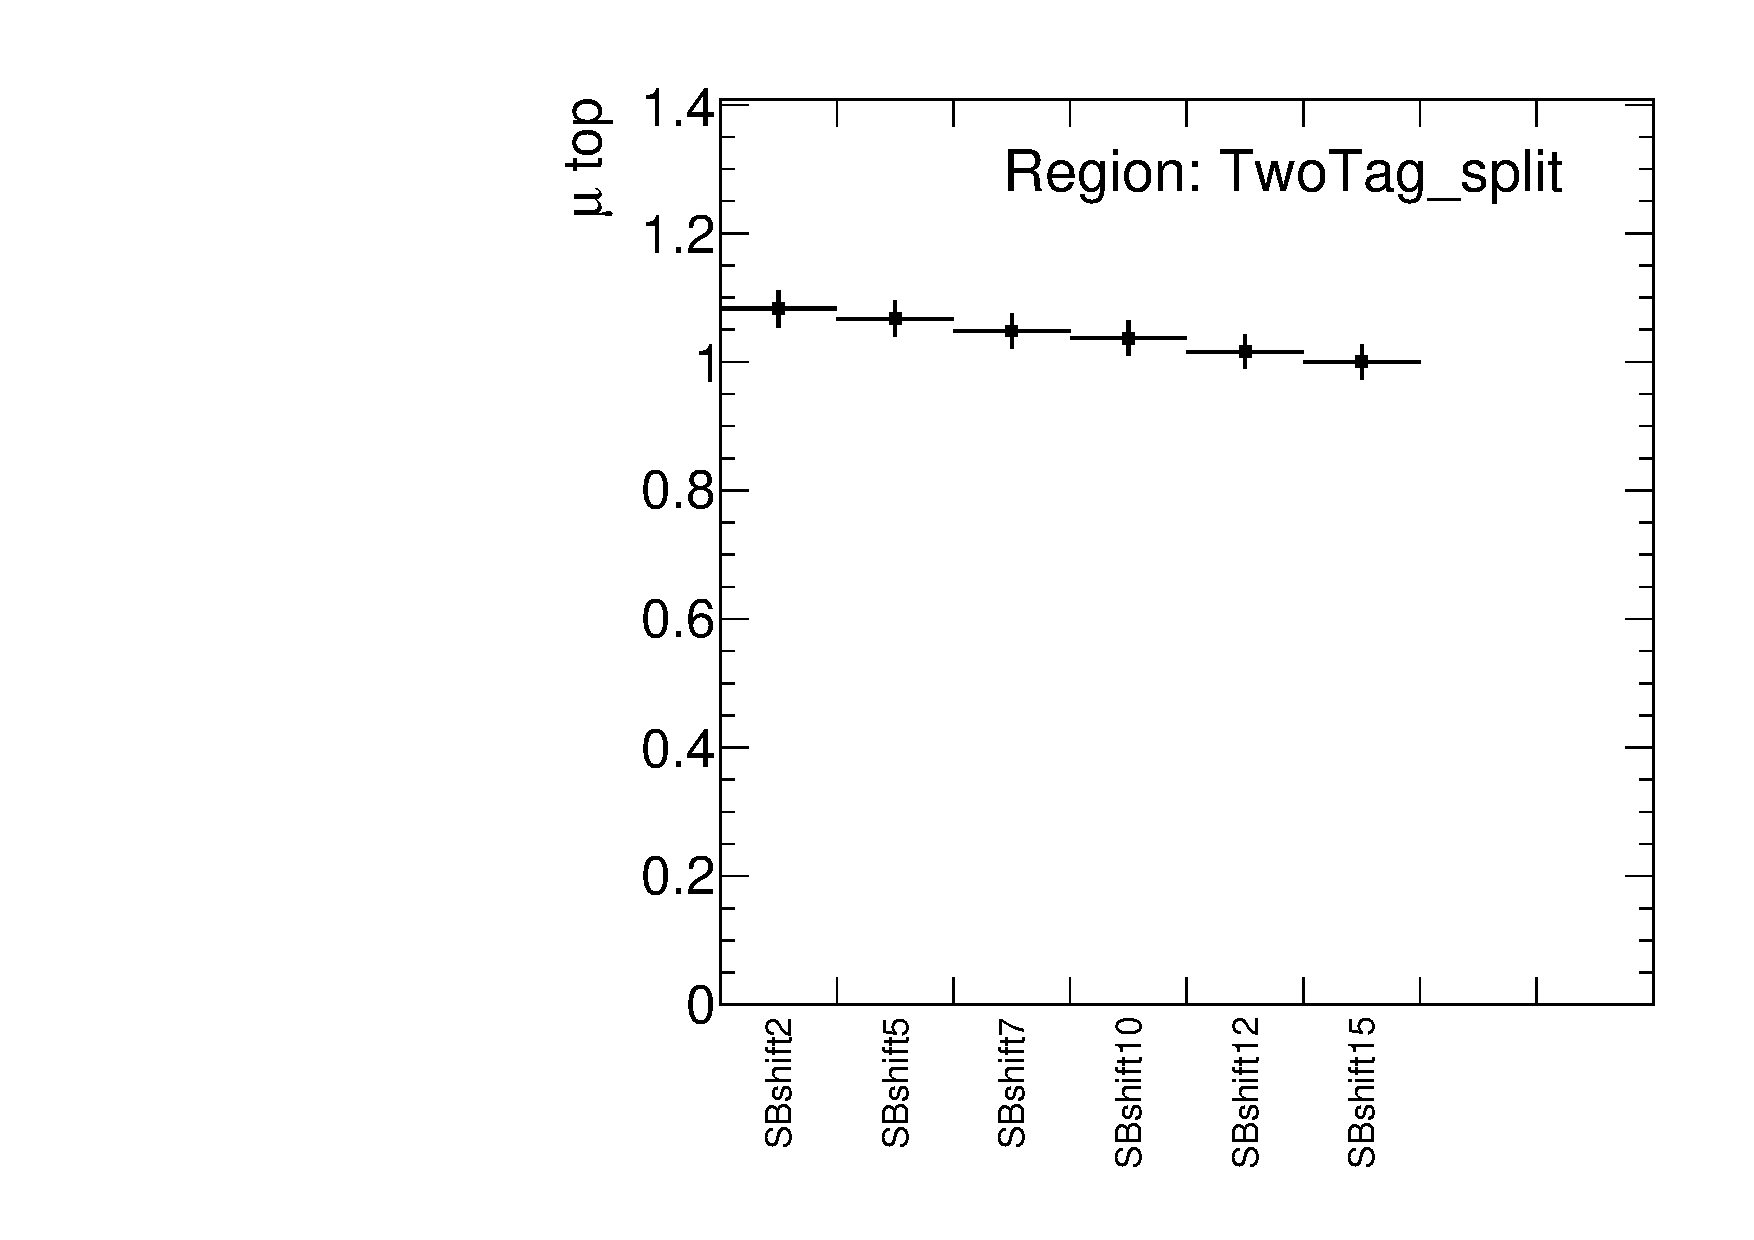
\includegraphics[angle=270, width=0.3\textwidth]{./figures/boosted/Appendix_SB/TwoTag_split_mutopSBshift.pdf}
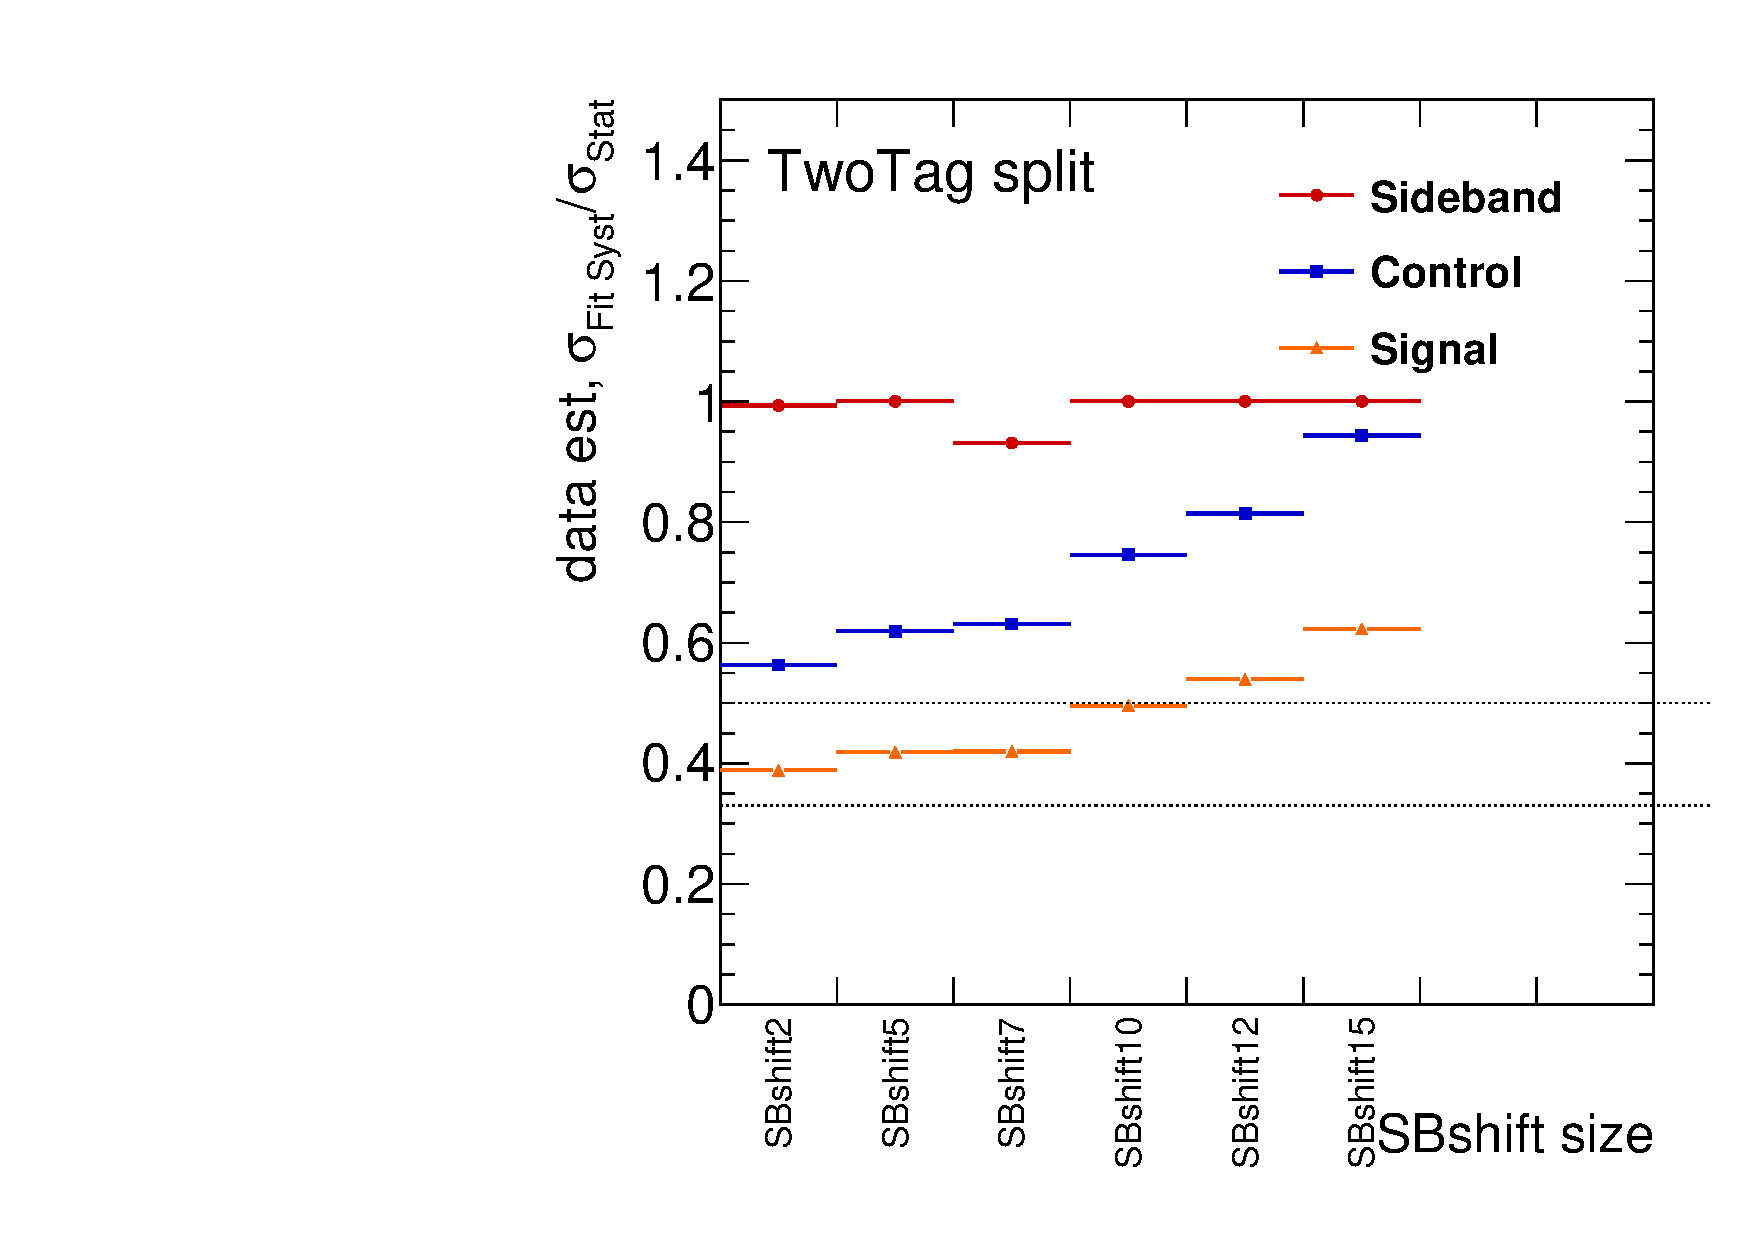
\includegraphics[angle=270, width=0.33\textwidth]{./figures/boosted/Appendix_SB/data_est_TwoTag_split_sigma_compareSBshift.pdf}
  \caption{Fit parameters for $\mu_{\text{qcd}}$ (left), $\alpha_{t\bar{t}}$ (middle), and ratio of fit uncertainty and stat uncertainty as a functioin of different Sideband shift values (right) , for 4$b$ (top) 3$b$ (middle) and 2$b$s (bottom). The Sideband region is chose to be $R_{hh}^{high} < 58$ with different shifts, and Control region is fixed at $33 < R_{hh}$. The x-axis indicates different values of SB center shifts.}
  \label{fig:app-sb-muqcd-diffSBshift}
\end{center}
\end{figure*}

\paragraph{} A similar test can be done on different Control Region sizes. This is shown in Figure~\ref{fig:app-sb-muqcd-diffCR}. Based on the choice that for the signal region predictions, the fit uncertainty should be around half of the statistical uncertainty, the Control upper limit is chosen to be $R_{hh} < 33$ \GeV.

\begin{figure*}[htbp!]
\begin{center}
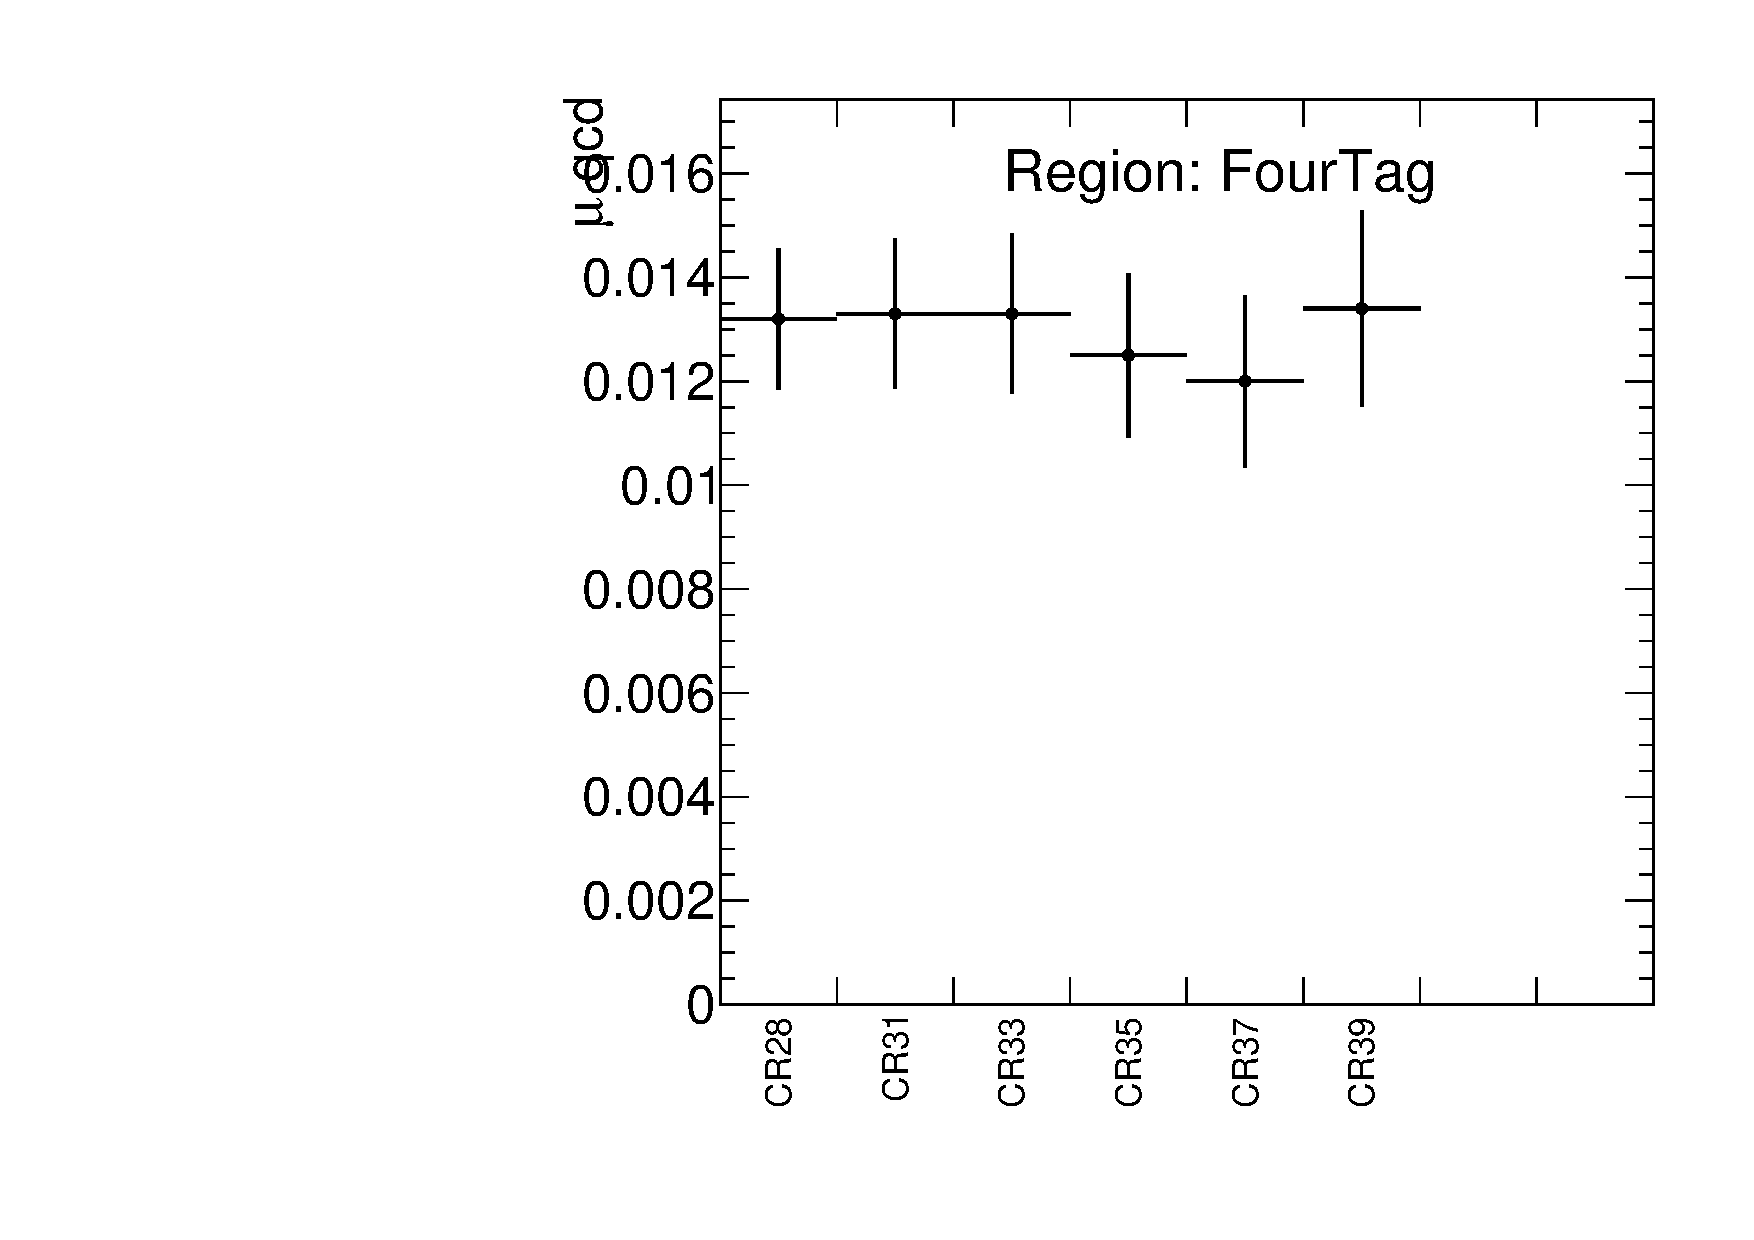
\includegraphics[angle=270, width=0.3\textwidth]{./figures/boosted/Appendix_SB/FourTag_muqcdCR.pdf}
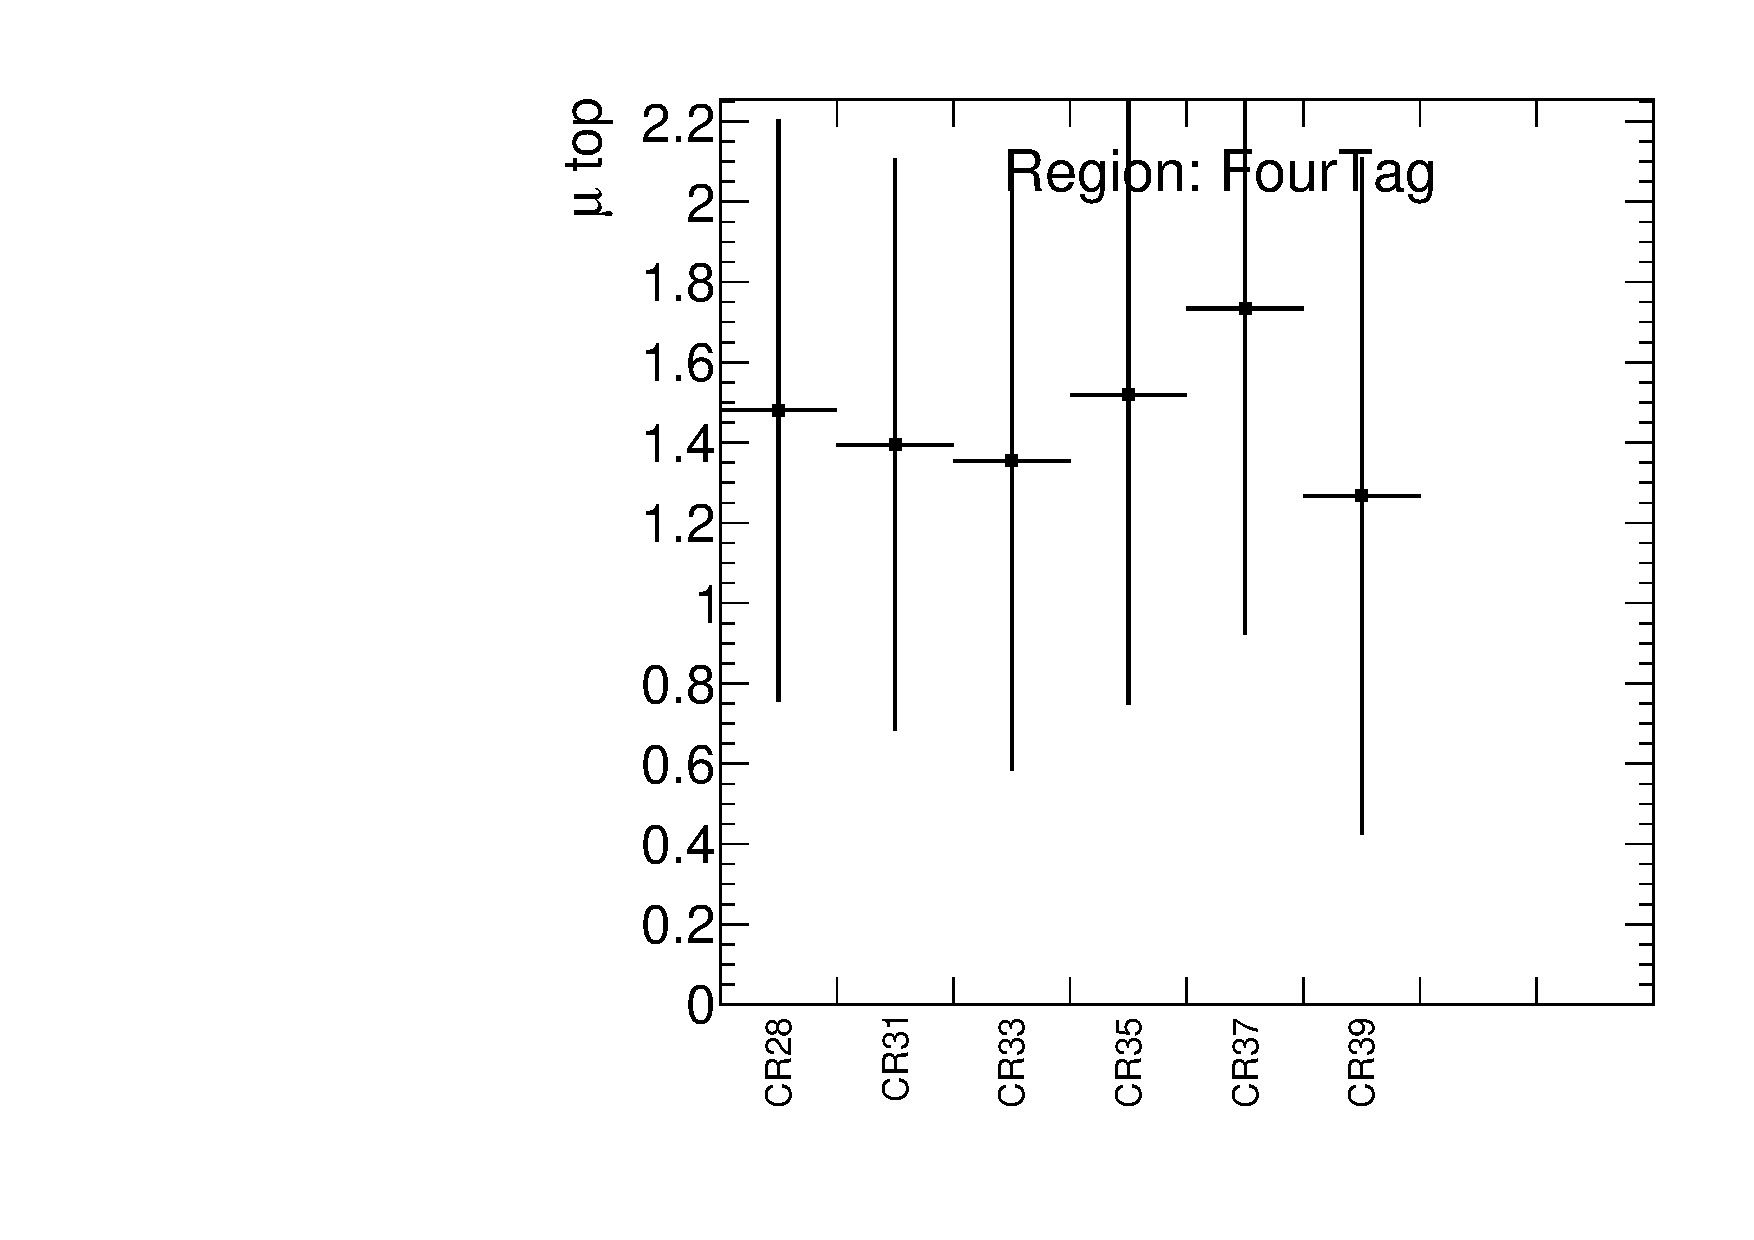
\includegraphics[angle=270, width=0.3\textwidth]{./figures/boosted/Appendix_SB/FourTag_mutopCR.pdf}
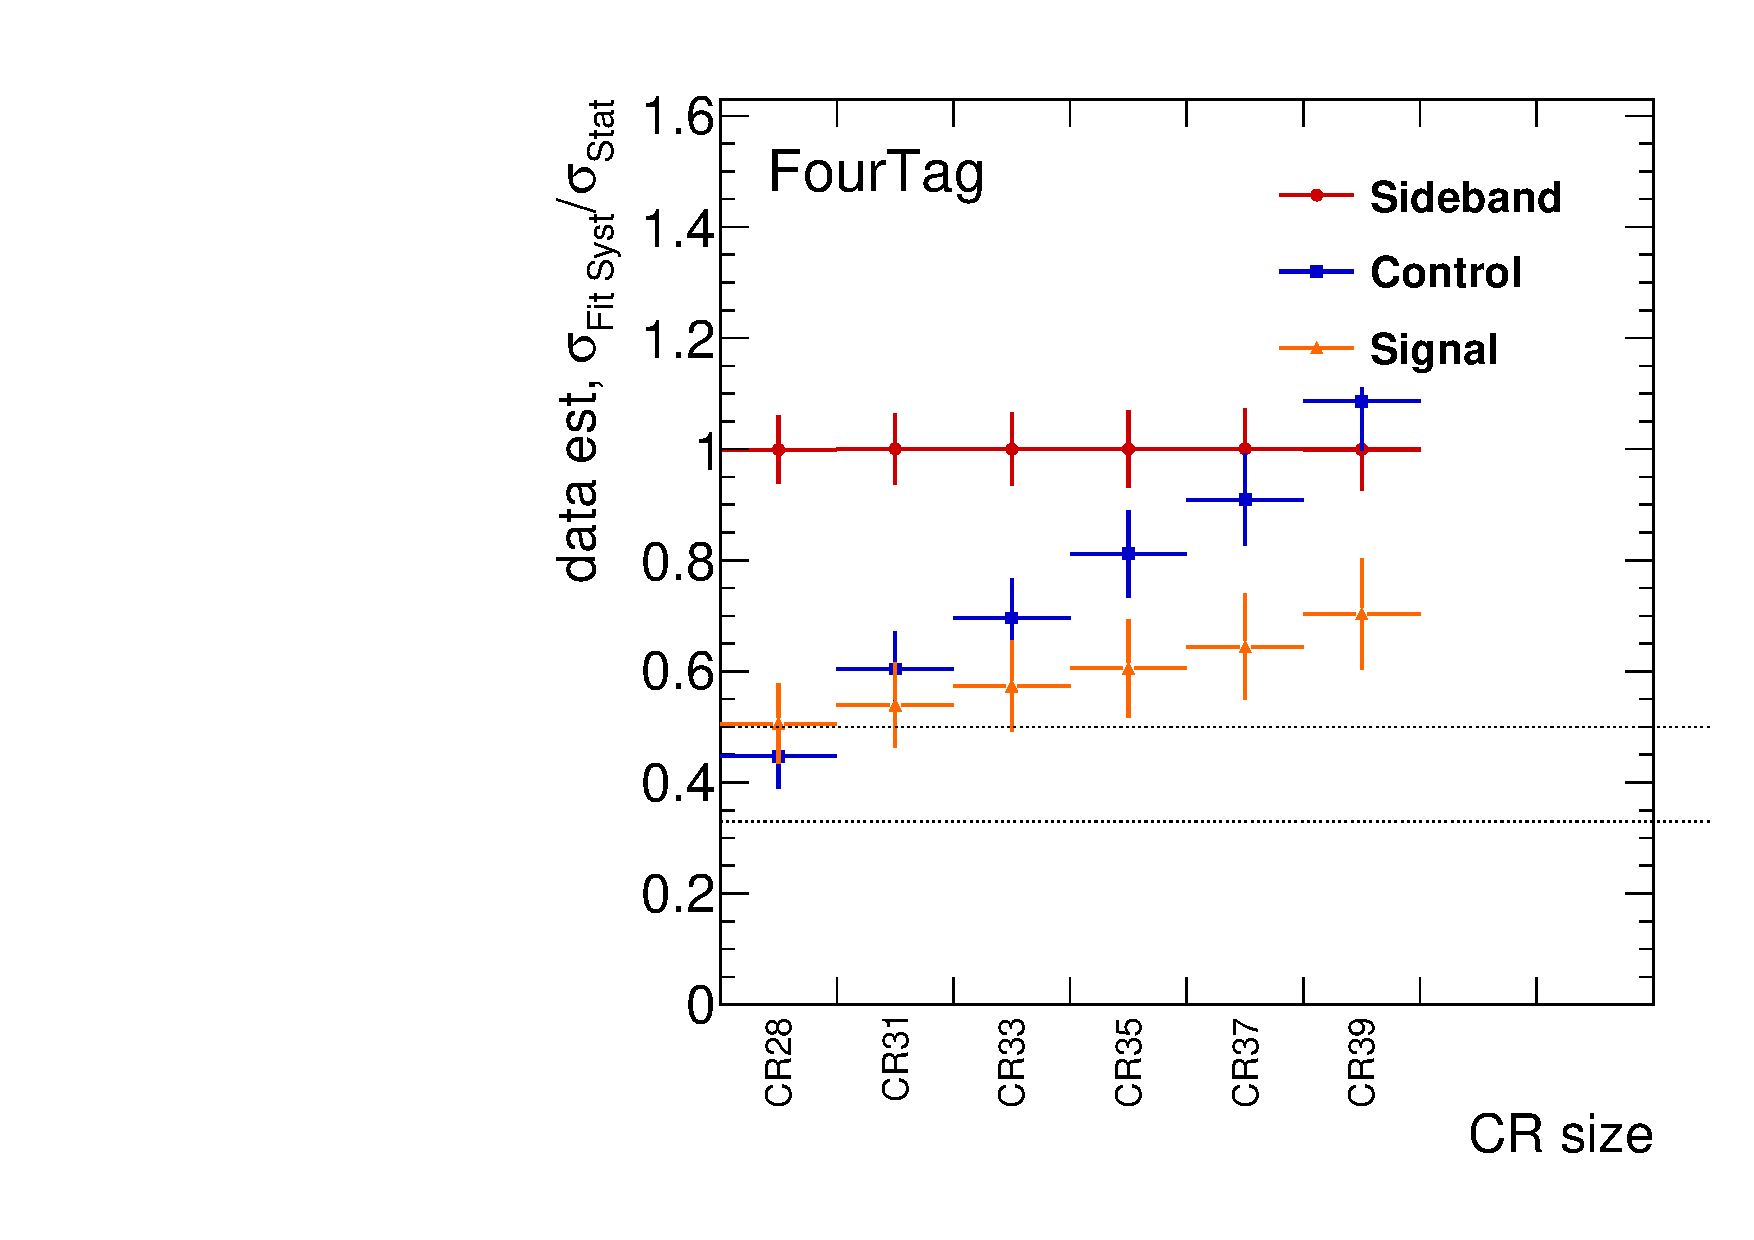
\includegraphics[angle=270, width=0.33\textwidth]{./figures/boosted/Appendix_SB/data_est_FourTag_sigma_compareCR.pdf}\\
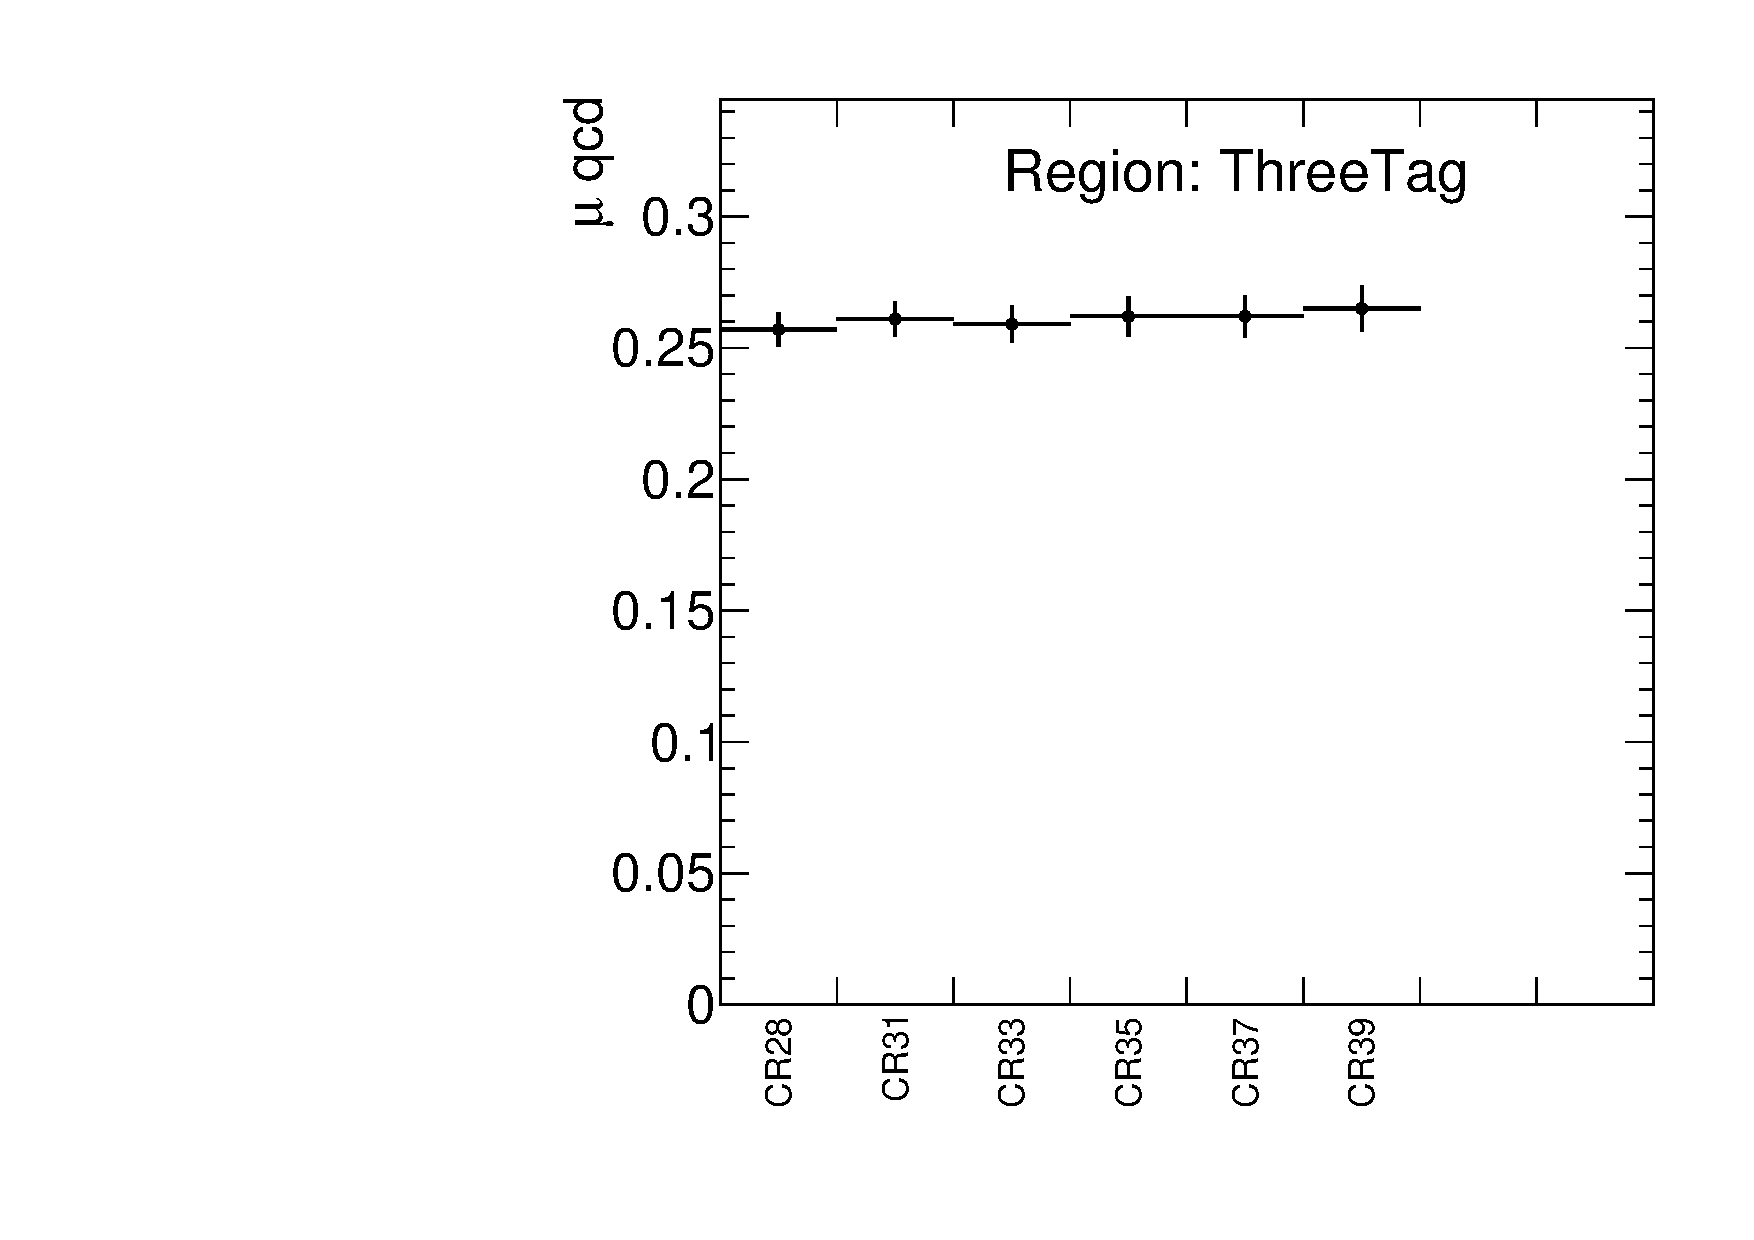
\includegraphics[angle=270, width=0.3\textwidth]{./figures/boosted/Appendix_SB/ThreeTag_muqcdCR.pdf}
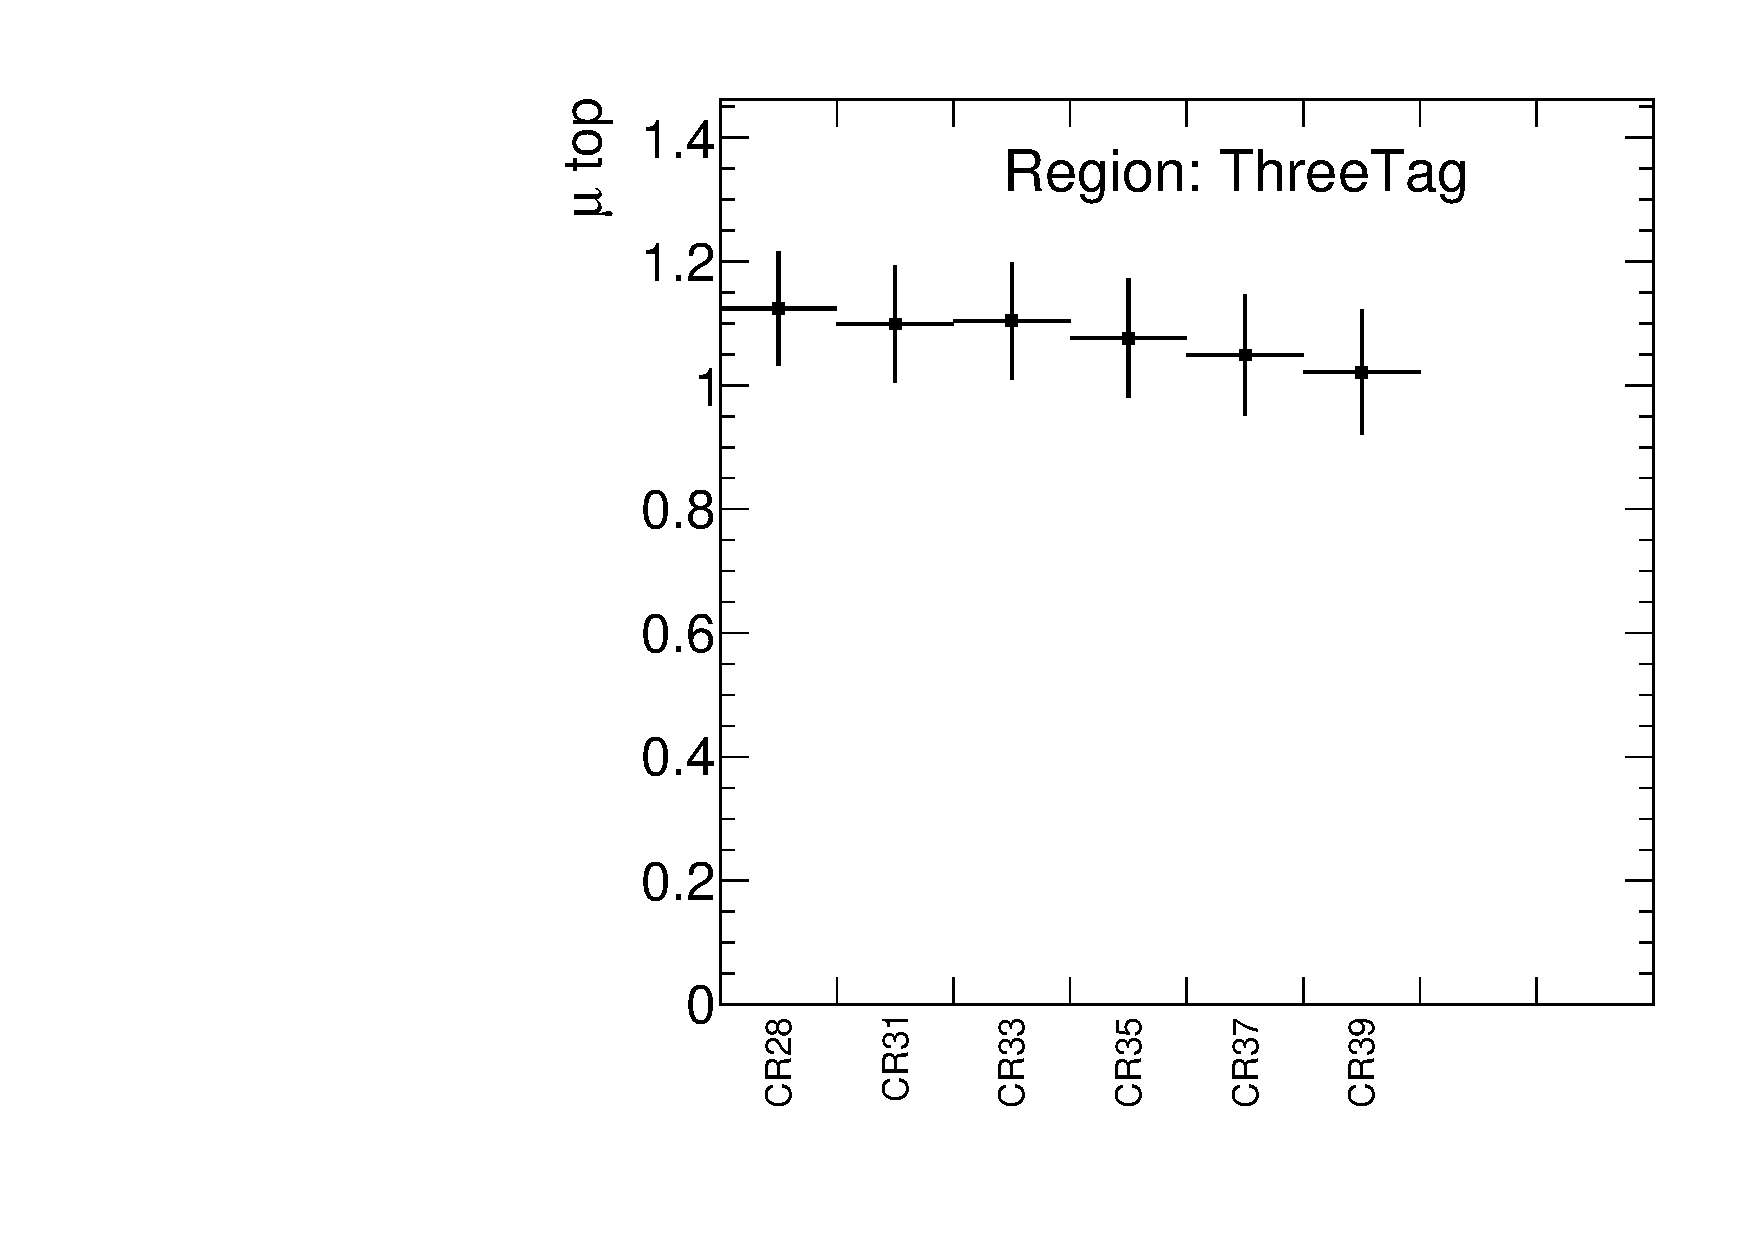
\includegraphics[angle=270, width=0.3\textwidth]{./figures/boosted/Appendix_SB/ThreeTag_mutopCR.pdf}
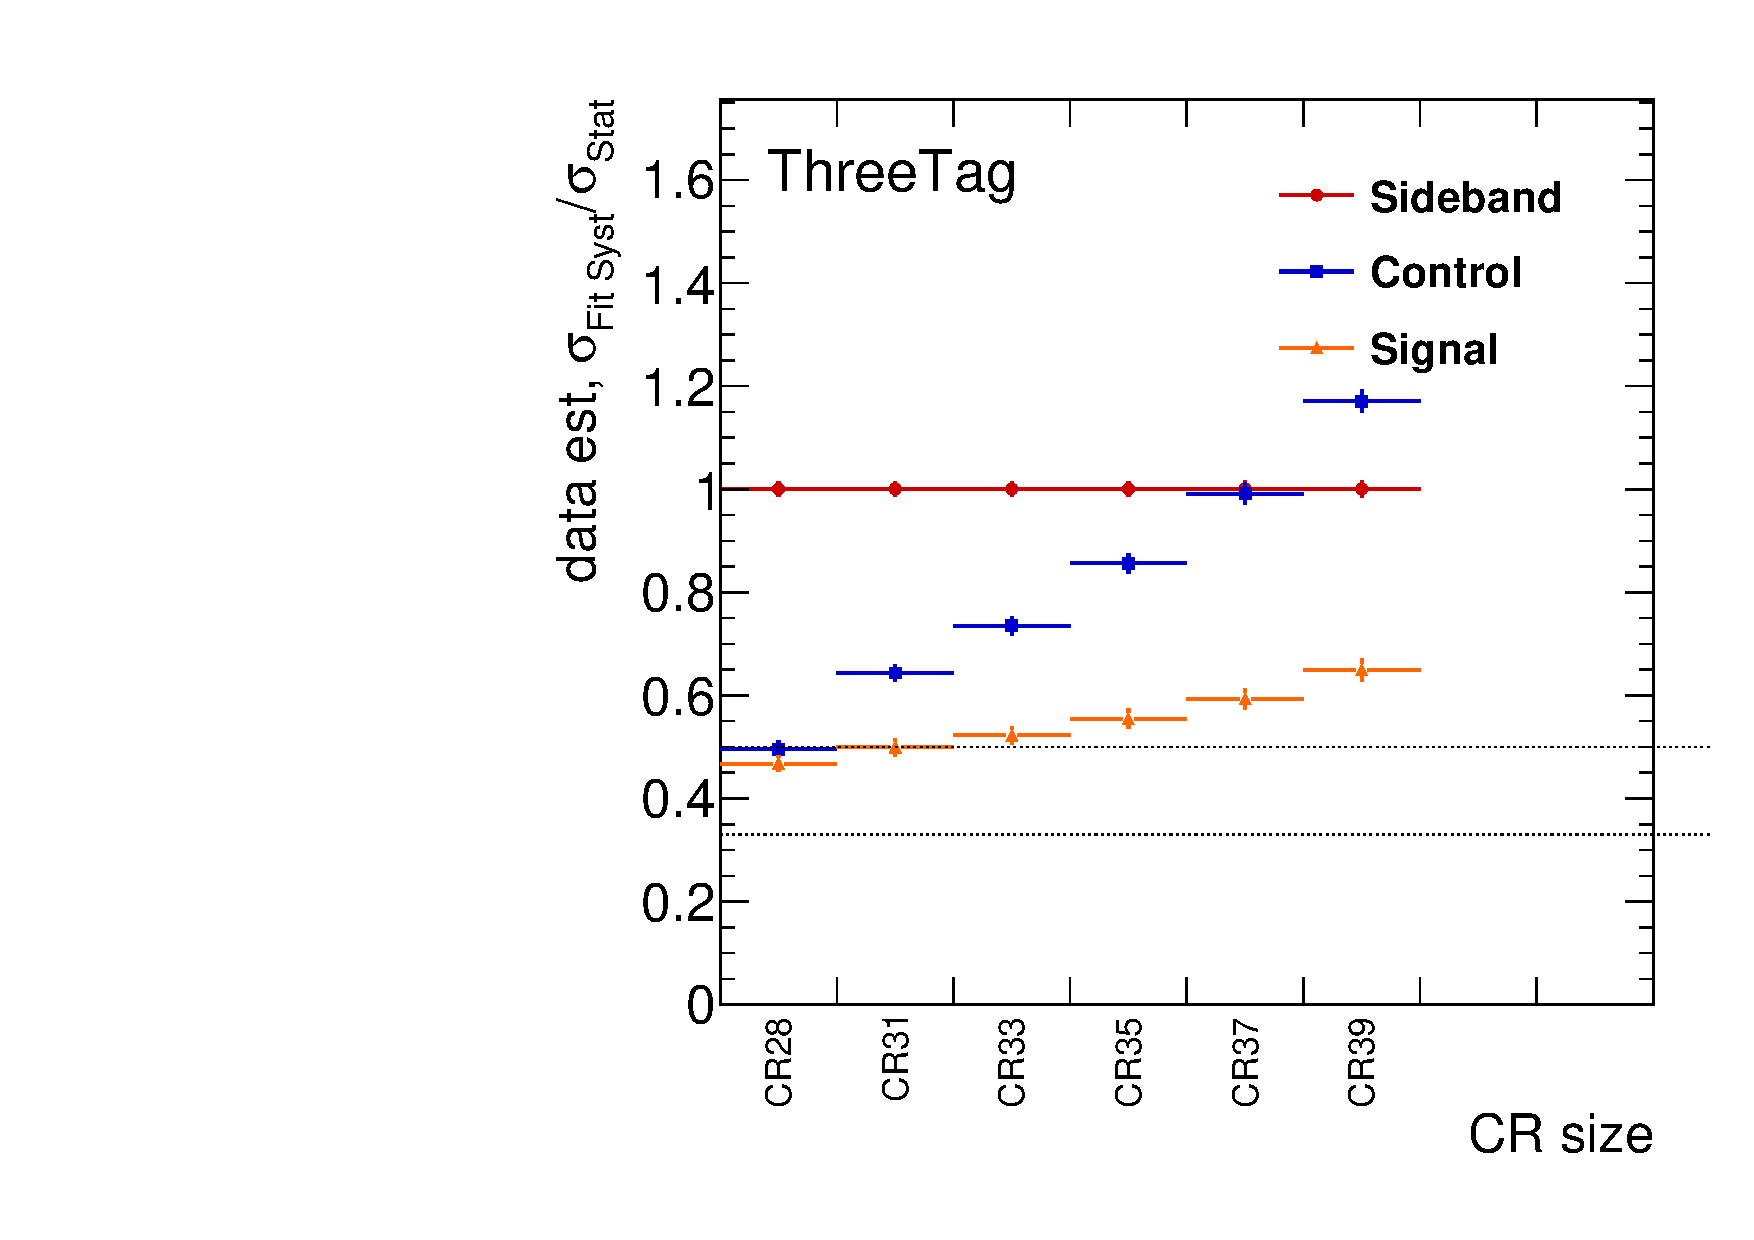
\includegraphics[angle=270, width=0.33\textwidth]{./figures/boosted/Appendix_SB/data_est_ThreeTag_sigma_compareCR.pdf}\\
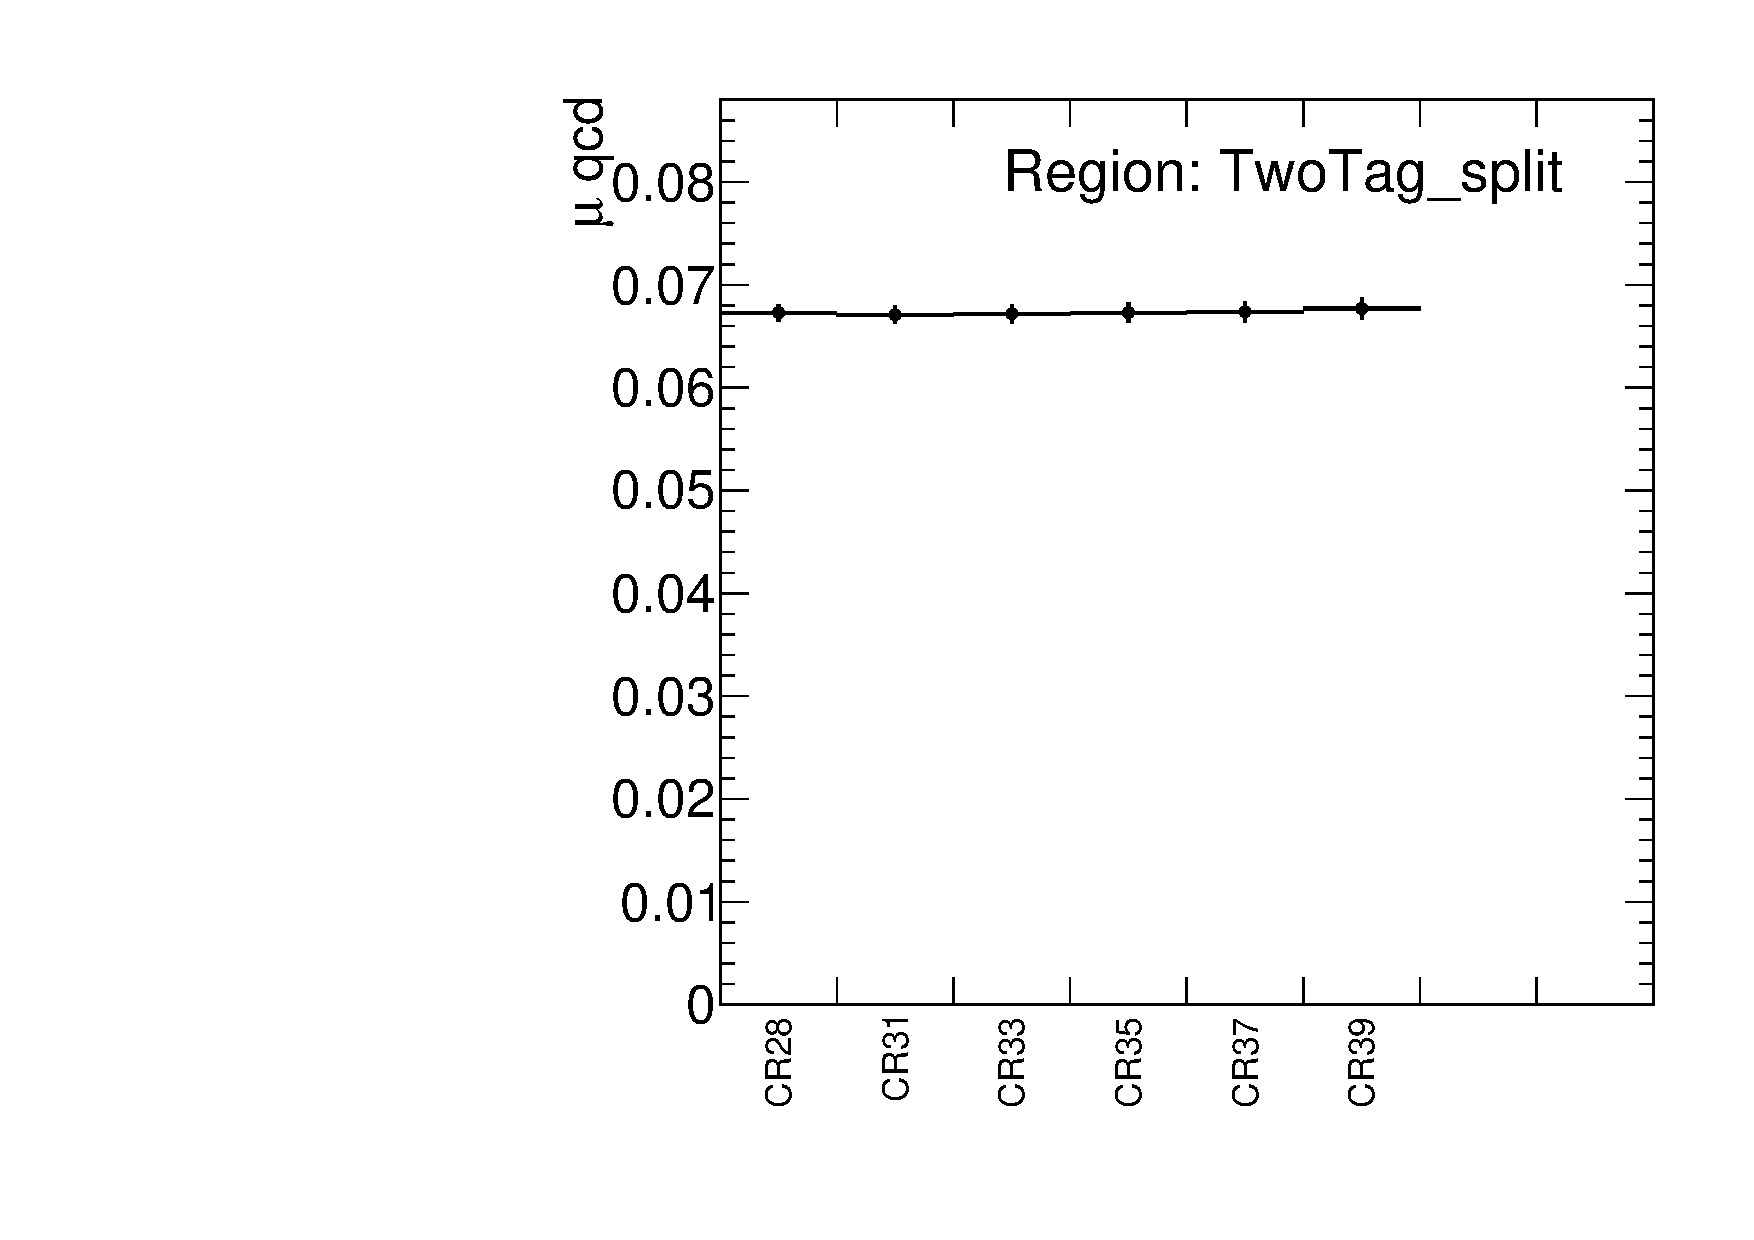
\includegraphics[angle=270, width=0.3\textwidth]{./figures/boosted/Appendix_SB/TwoTag_split_muqcdCR.pdf}
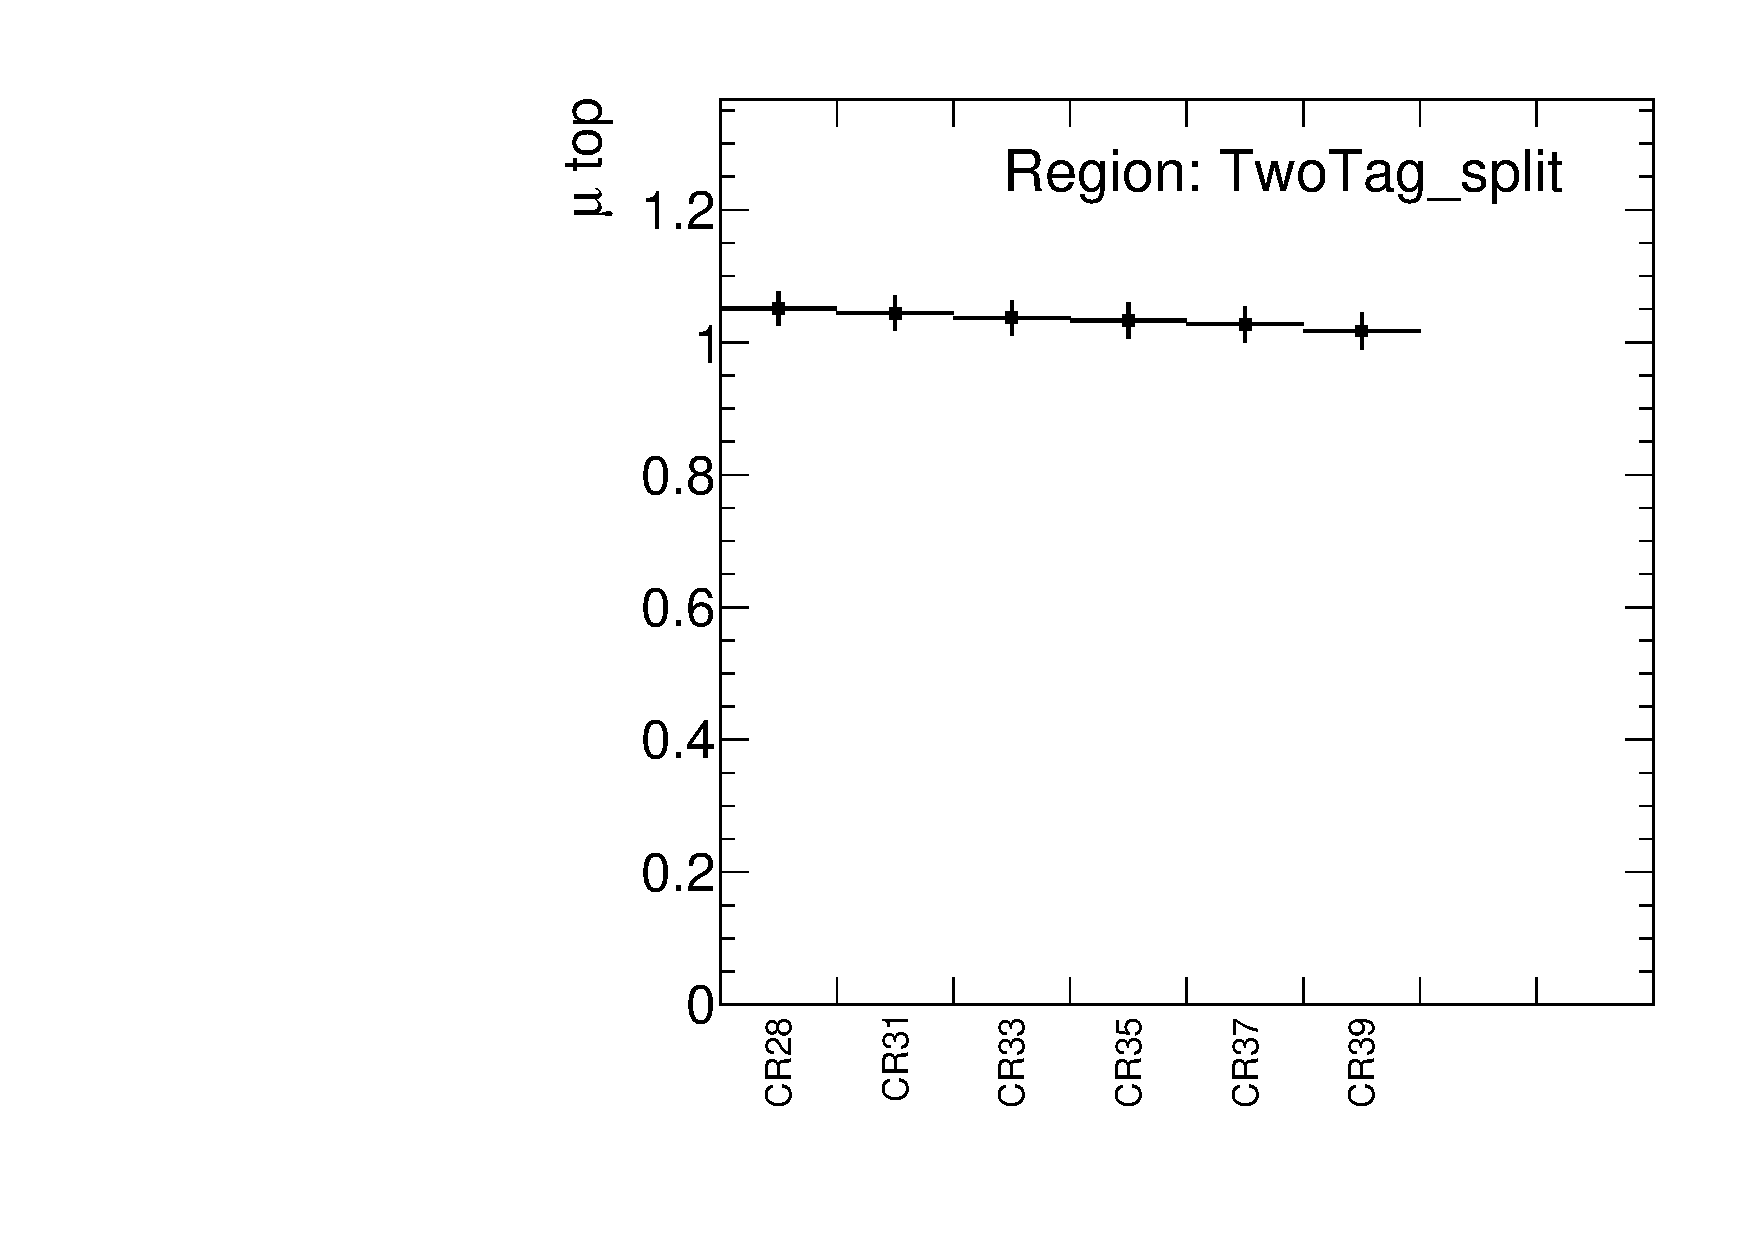
\includegraphics[angle=270, width=0.3\textwidth]{./figures/boosted/Appendix_SB/TwoTag_split_mutopCR.pdf}
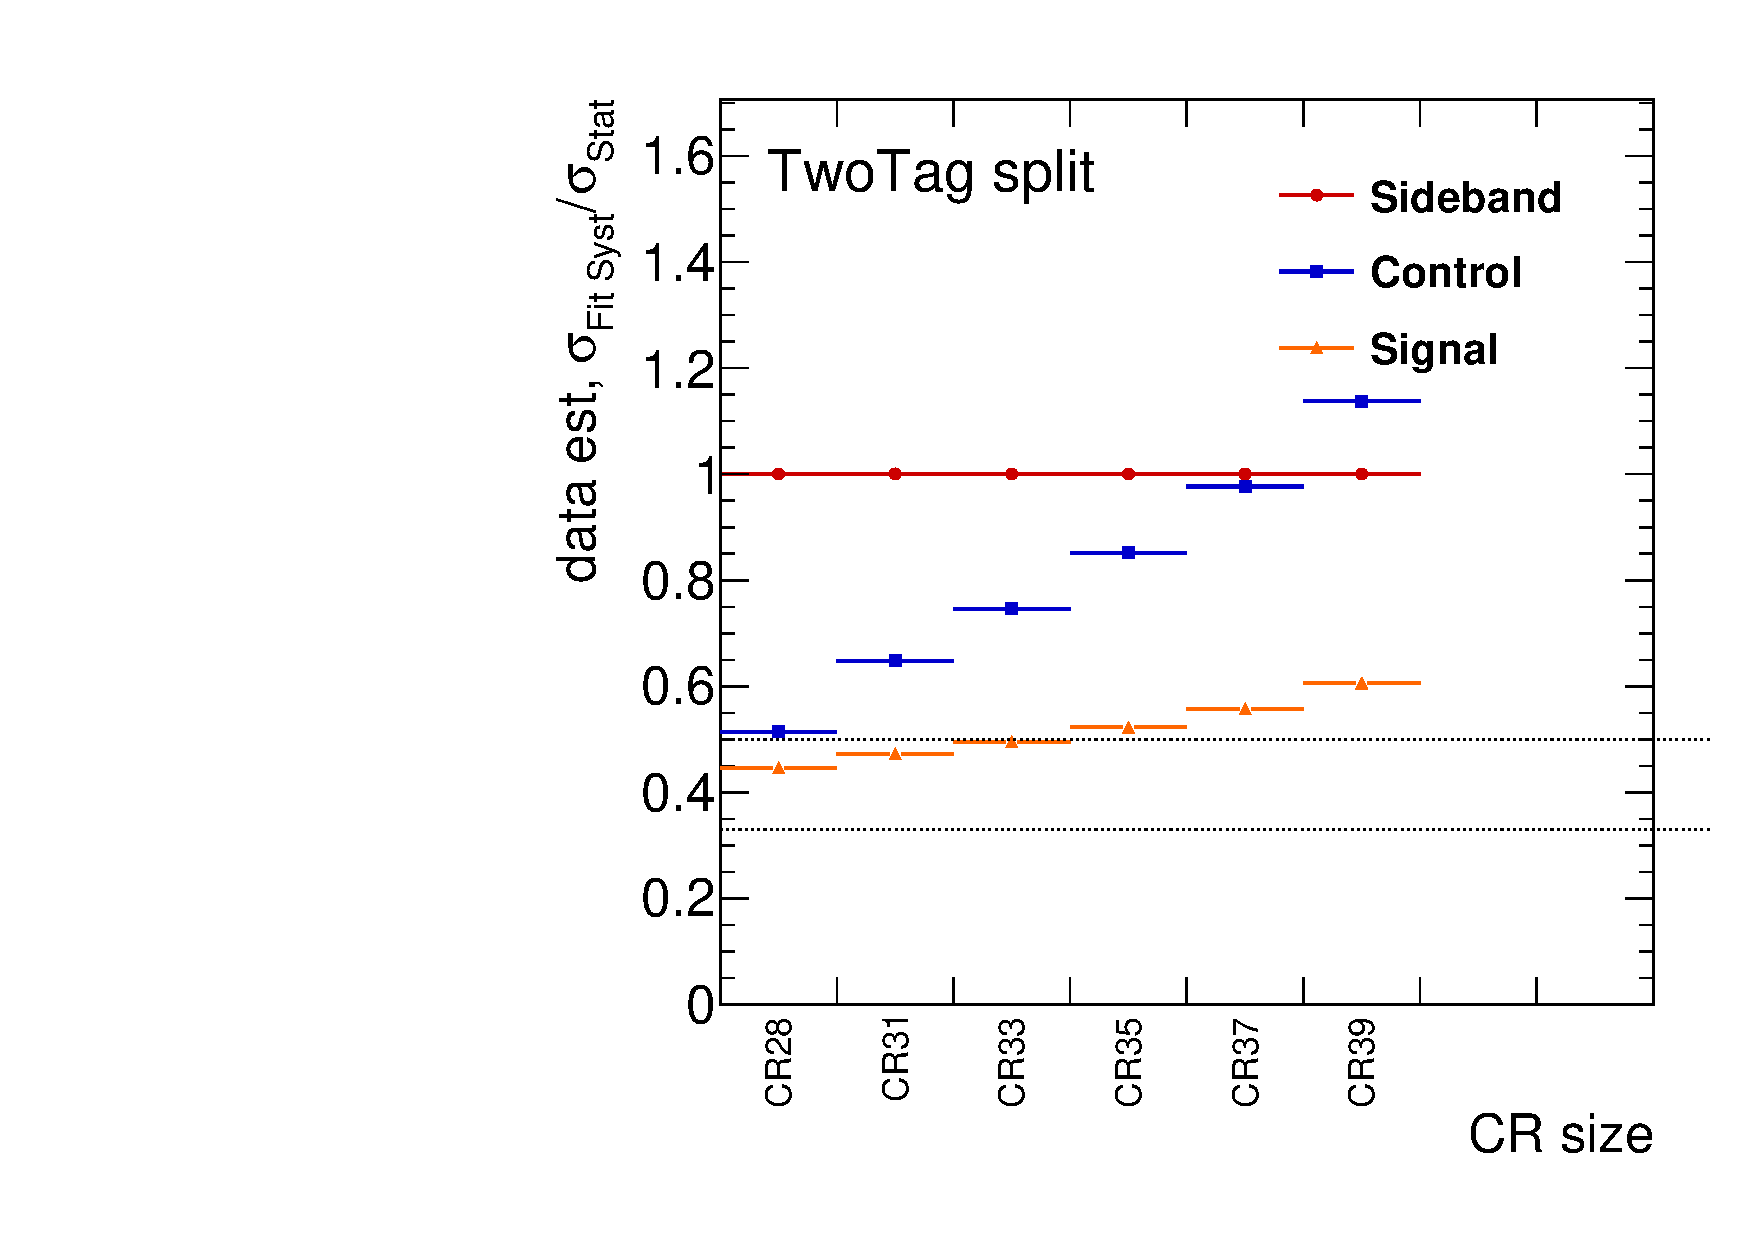
\includegraphics[angle=270, width=0.33\textwidth]{./figures/boosted/Appendix_SB/data_est_TwoTag_split_sigma_compareCR.pdf}
  \caption{Fit parameters for $\mu_{\text{qcd}}$ (left), $\alpha_{t\bar{t}}$ (middle), and ratio of fit uncertainty and stat uncertainty as a functioin of different Control values (right) , for 4$b$ (top) 3$b$ (middle) and 2$b$s (bottom). The Sideband is chosen to be $R_{hh}^{high} < 58$ with 10 \GeV shifts. The x-axis indicates different values of CR $R_{hh}$ cuts.}
  \label{fig:app-sb-muqcd-diffCR}
\end{center}
\end{figure*}
